% Options for packages loaded elsewhere
\PassOptionsToPackage{unicode}{hyperref}
\PassOptionsToPackage{hyphens}{url}
%
\documentclass[
  11pt,
]{article}
\usepackage{lmodern}
\usepackage{amssymb,amsmath}
\usepackage{ifxetex,ifluatex}
\ifnum 0\ifxetex 1\fi\ifluatex 1\fi=0 % if pdftex
  \usepackage[T1]{fontenc}
  \usepackage[utf8]{inputenc}
  \usepackage{textcomp} % provide euro and other symbols
\else % if luatex or xetex
  \usepackage{unicode-math}
  \defaultfontfeatures{Scale=MatchLowercase}
  \defaultfontfeatures[\rmfamily]{Ligatures=TeX,Scale=1}
\fi
% Use upquote if available, for straight quotes in verbatim environments
\IfFileExists{upquote.sty}{\usepackage{upquote}}{}
\IfFileExists{microtype.sty}{% use microtype if available
  \usepackage[]{microtype}
  \UseMicrotypeSet[protrusion]{basicmath} % disable protrusion for tt fonts
}{}
\makeatletter
\@ifundefined{KOMAClassName}{% if non-KOMA class
  \IfFileExists{parskip.sty}{%
    \usepackage{parskip}
  }{% else
    \setlength{\parindent}{0pt}
    \setlength{\parskip}{6pt plus 2pt minus 1pt}}
}{% if KOMA class
  \KOMAoptions{parskip=half}}
\makeatother
\usepackage{xcolor}
\IfFileExists{xurl.sty}{\usepackage{xurl}}{} % add URL line breaks if available
\IfFileExists{bookmark.sty}{\usepackage{bookmark}}{\usepackage{hyperref}}
\hypersetup{
  pdftitle={Appendix S2. Summarize S/R model results and compute management reference points},
  hidelinks,
  pdfcreator={LaTeX via pandoc}}
\urlstyle{same} % disable monospaced font for URLs
\usepackage[margin=1in]{geometry}
\usepackage{color}
\usepackage{fancyvrb}
\newcommand{\VerbBar}{|}
\newcommand{\VERB}{\Verb[commandchars=\\\{\}]}
\DefineVerbatimEnvironment{Highlighting}{Verbatim}{commandchars=\\\{\}}
% Add ',fontsize=\small' for more characters per line
\newenvironment{Shaded}{}{}
\newcommand{\AlertTok}[1]{\textcolor[rgb]{1.00,0.00,0.00}{#1}}
\newcommand{\AnnotationTok}[1]{\textcolor[rgb]{0.00,0.50,0.00}{#1}}
\newcommand{\AttributeTok}[1]{#1}
\newcommand{\BaseNTok}[1]{#1}
\newcommand{\BuiltInTok}[1]{#1}
\newcommand{\CharTok}[1]{\textcolor[rgb]{0.00,0.50,0.50}{#1}}
\newcommand{\CommentTok}[1]{\textcolor[rgb]{0.00,0.50,0.00}{#1}}
\newcommand{\CommentVarTok}[1]{\textcolor[rgb]{0.00,0.50,0.00}{#1}}
\newcommand{\ConstantTok}[1]{#1}
\newcommand{\ControlFlowTok}[1]{\textcolor[rgb]{0.00,0.00,1.00}{#1}}
\newcommand{\DataTypeTok}[1]{#1}
\newcommand{\DecValTok}[1]{#1}
\newcommand{\DocumentationTok}[1]{\textcolor[rgb]{0.00,0.50,0.00}{#1}}
\newcommand{\ErrorTok}[1]{\textcolor[rgb]{1.00,0.00,0.00}{\textbf{#1}}}
\newcommand{\ExtensionTok}[1]{#1}
\newcommand{\FloatTok}[1]{#1}
\newcommand{\FunctionTok}[1]{#1}
\newcommand{\ImportTok}[1]{#1}
\newcommand{\InformationTok}[1]{\textcolor[rgb]{0.00,0.50,0.00}{#1}}
\newcommand{\KeywordTok}[1]{\textcolor[rgb]{0.00,0.00,1.00}{#1}}
\newcommand{\NormalTok}[1]{#1}
\newcommand{\OperatorTok}[1]{#1}
\newcommand{\OtherTok}[1]{\textcolor[rgb]{1.00,0.25,0.00}{#1}}
\newcommand{\PreprocessorTok}[1]{\textcolor[rgb]{1.00,0.25,0.00}{#1}}
\newcommand{\RegionMarkerTok}[1]{#1}
\newcommand{\SpecialCharTok}[1]{\textcolor[rgb]{0.00,0.50,0.50}{#1}}
\newcommand{\SpecialStringTok}[1]{\textcolor[rgb]{0.00,0.50,0.50}{#1}}
\newcommand{\StringTok}[1]{\textcolor[rgb]{0.00,0.50,0.50}{#1}}
\newcommand{\VariableTok}[1]{#1}
\newcommand{\VerbatimStringTok}[1]{\textcolor[rgb]{0.00,0.50,0.50}{#1}}
\newcommand{\WarningTok}[1]{\textcolor[rgb]{0.00,0.50,0.00}{\textbf{#1}}}
\usepackage{graphicx,grffile}
\makeatletter
\def\maxwidth{\ifdim\Gin@nat@width>\linewidth\linewidth\else\Gin@nat@width\fi}
\def\maxheight{\ifdim\Gin@nat@height>\textheight\textheight\else\Gin@nat@height\fi}
\makeatother
% Scale images if necessary, so that they will not overflow the page
% margins by default, and it is still possible to overwrite the defaults
% using explicit options in \includegraphics[width, height, ...]{}
\setkeys{Gin}{width=\maxwidth,height=\maxheight,keepaspectratio}
% Set default figure placement to htbp
\makeatletter
\def\fps@figure{htbp}
\makeatother
\setlength{\emergencystretch}{3em} % prevent overfull lines
\providecommand{\tightlist}{%
  \setlength{\itemsep}{0pt}\setlength{\parskip}{0pt}}
\setcounter{secnumdepth}{5}

\title{Appendix S2. Summarize S/R model results and compute management
reference points}
\usepackage{etoolbox}
\makeatletter
\providecommand{\subtitle}[1]{% add subtitle to \maketitle
  \apptocmd{\@title}{\par {\large #1 \par}}{}{}
}
\makeatother
\subtitle{2021 Skagit River Spring Chinook RER.}
\author{}
\date{\vspace{-2.5em}}

\begin{document}
\maketitle

{
\setcounter{tocdepth}{3}
\tableofcontents
}
\vspace{0.2in}

This is version 0.24.08.26.

\hypertarget{background}{%
\section{Background}\label{background}}

This appendix shows how generate model averaged parameter estimates and
generate figures relevant to the 2020-2021 wild Skagit River steelhead
forecast. All analyses require the \href{https://cran.r-project.org/}{R
software} (v3.5 or later), as well as a few packages that are not
included with the base installation of R.

\begin{Shaded}
\begin{Highlighting}[]
\ControlFlowTok{if}\NormalTok{(}\OperatorTok{!}\KeywordTok{require}\NormalTok{(}\StringTok{"readr"}\NormalTok{)) \{}
  \KeywordTok{install.packages}\NormalTok{(}\StringTok{"readr"}\NormalTok{)}
  \KeywordTok{library}\NormalTok{(}\StringTok{"readr"}\NormalTok{)}
\NormalTok{\}}
\ControlFlowTok{if}\NormalTok{(}\OperatorTok{!}\KeywordTok{require}\NormalTok{(}\StringTok{"captioner"}\NormalTok{)) \{}
\NormalTok{  devtools}\OperatorTok{::}\KeywordTok{install_github}\NormalTok{(}\StringTok{"adletaw/captioner"}\NormalTok{)}
  \KeywordTok{library}\NormalTok{(}\StringTok{"captioner"}\NormalTok{)}
\NormalTok{\}}
\ControlFlowTok{if}\NormalTok{(}\OperatorTok{!}\KeywordTok{require}\NormalTok{(}\StringTok{"coda"}\NormalTok{)) \{}
  \KeywordTok{install.packages}\NormalTok{(}\StringTok{"coda"}\NormalTok{)}
  \KeywordTok{library}\NormalTok{(}\StringTok{"coda"}\NormalTok{)}
\NormalTok{\}}
\ControlFlowTok{if}\NormalTok{(}\OperatorTok{!}\KeywordTok{require}\NormalTok{(}\StringTok{"here"}\NormalTok{)) \{}
  \KeywordTok{install.packages}\NormalTok{(}\StringTok{"here"}\NormalTok{)}
  \KeywordTok{library}\NormalTok{(}\StringTok{"here"}\NormalTok{)}
\NormalTok{\}}
\ControlFlowTok{if}\NormalTok{(}\OperatorTok{!}\KeywordTok{require}\NormalTok{(}\StringTok{"gsl"}\NormalTok{)) \{}
  \KeywordTok{install.packages}\NormalTok{(}\StringTok{"gsl"}\NormalTok{)}
  \KeywordTok{library}\NormalTok{(}\StringTok{"gsl"}\NormalTok{)}
\NormalTok{\}}
\ControlFlowTok{if}\NormalTok{(}\OperatorTok{!}\KeywordTok{require}\NormalTok{(}\StringTok{"loo"}\NormalTok{)) \{}
  \KeywordTok{install.packages}\NormalTok{(}\StringTok{"loo"}\NormalTok{)}
  \KeywordTok{library}\NormalTok{(}\StringTok{"loo"}\NormalTok{)}
\NormalTok{\}}

\CommentTok{## set default caption delimter}
\NormalTok{fig_cap <-}\StringTok{ }\KeywordTok{captioner}\NormalTok{(}\DataTypeTok{infix =} \StringTok{"."}\NormalTok{)}

\NormalTok{management_unit <-}\StringTok{ "spring"}

\CommentTok{## set directory locations}
\NormalTok{datadir <-}\StringTok{ }\KeywordTok{here}\NormalTok{(}\KeywordTok{paste}\NormalTok{(management_unit,}\StringTok{"/"}\NormalTok{,}\StringTok{"data"}\NormalTok{,}\DataTypeTok{sep =} \StringTok{""}\NormalTok{))}
\NormalTok{jagsdir <-}\StringTok{ }\KeywordTok{here}\NormalTok{(}\KeywordTok{paste}\NormalTok{(management_unit,}\StringTok{"/"}\NormalTok{,}\StringTok{"jags"}\NormalTok{,}\DataTypeTok{sep =} \StringTok{""}\NormalTok{))}
\NormalTok{analdir <-}\StringTok{ }\KeywordTok{here}\NormalTok{(}\KeywordTok{paste}\NormalTok{(management_unit,}\StringTok{"/"}\NormalTok{,}\StringTok{"analysis"}\NormalTok{,}\DataTypeTok{sep =} \StringTok{""}\NormalTok{))}
\NormalTok{savedir <-}\StringTok{ }\KeywordTok{here}\NormalTok{(}\KeywordTok{paste}\NormalTok{(management_unit,}\StringTok{"/"}\NormalTok{,}\StringTok{"analysis/cache"}\NormalTok{,}\DataTypeTok{sep =} \StringTok{""}\NormalTok{))}

\CommentTok{## better round/floor/ceiling}
\NormalTok{around <-}\StringTok{ }\ControlFlowTok{function}\NormalTok{(x, }\DataTypeTok{func =} \StringTok{"round"}\NormalTok{, }\DataTypeTok{prec =} \DecValTok{1}\NormalTok{) \{}
  \CommentTok{## `func` can be "round", "floor", or "ceiling"}
  \CommentTok{## `prec` is desired precision (eg, 0.1 is to nearest tenth)}
  \ControlFlowTok{if}\NormalTok{(}\OperatorTok{!}\KeywordTok{is.double}\NormalTok{(x)) \{}
    \KeywordTok{stop}\NormalTok{(}\StringTok{"`x` must be a real number"}\NormalTok{)}
\NormalTok{  \}}
  \ControlFlowTok{if}\NormalTok{(}\OperatorTok{!}\NormalTok{(func }\OperatorTok\StringTok{ }\KeywordTok{c}\NormalTok{(}\StringTok{"round"}\NormalTok{, }\StringTok{"floor"}\NormalTok{, }\StringTok{"ceiling"}\NormalTok{))) \{}
    \KeywordTok{stop}\NormalTok{(}\StringTok{"`func` must be }\CharTok{\textbackslash{}"}\StringTok{round}\CharTok{\textbackslash{}"}\StringTok{, }\CharTok{\textbackslash{}"}\StringTok{floor}\CharTok{\textbackslash{}"}\StringTok{, or }\CharTok{\textbackslash{}"}\StringTok{ceiling}\CharTok{\textbackslash{}"}\StringTok{"}\NormalTok{)}
\NormalTok{  \}}
  \ControlFlowTok{if}\NormalTok{(prec }\OperatorTok{<=}\StringTok{ }\DecValTok{0}\NormalTok{) \{}
    \KeywordTok{stop}\NormalTok{(}\StringTok{"`prec` cannot be less than or equal to 0"}\NormalTok{)}
\NormalTok{  \}}
  \KeywordTok{do.call}\NormalTok{(func, }\KeywordTok{list}\NormalTok{(x }\OperatorTok{/}\StringTok{ }\NormalTok{prec)) }\OperatorTok{*}\StringTok{ }\NormalTok{prec}
\NormalTok{\}}

\CommentTok{#load complete model fits & model refits with subset data}
\NormalTok{loadmodfits<-}\ControlFlowTok{function}\NormalTok{(modelnames)\{}
\NormalTok{  mod_fits<-}\KeywordTok{list}\NormalTok{(}\OtherTok{NULL}\NormalTok{)}
  \ControlFlowTok{for}\NormalTok{(i }\ControlFlowTok{in} \DecValTok{1}\OperatorTok{:}\KeywordTok{length}\NormalTok{(modelnames))\{}
\NormalTok{    mod_fits[[i]] <-}\StringTok{ }\KeywordTok{readRDS}\NormalTok{(}\KeywordTok{file.path}\NormalTok{(savedir,}\KeywordTok{paste0}\NormalTok{(modelnames[i],}\StringTok{"_y"}\NormalTok{,n_forecasts}\OperatorTok{+}\DecValTok{1}\NormalTok{,}\StringTok{"_"}\NormalTok{,run,}\StringTok{".rds"}\NormalTok{)))}
    \CommentTok{#mod_fits[[i]] <- readRDS(file.path(savedir,paste0("fit_",modelnames[i],".rds")))}
\NormalTok{  \}}
  \KeywordTok{return}\NormalTok{(mod_fits)}
\NormalTok{\}}

\NormalTok{Re2prec <-}\StringTok{ }\ControlFlowTok{function}\NormalTok{(x,}\DataTypeTok{map=}\StringTok{"round"}\NormalTok{,}\DataTypeTok{prec=}\DecValTok{1}\NormalTok{) \{}
\CommentTok{## 'map' can be round, floor, or ceiling}
\CommentTok{## 'prec' is nearest value (eg, 0.1 means to nearest tenth); default 1 gives normal behavior}
\ControlFlowTok{if}\NormalTok{(prec}\OperatorTok{<=}\DecValTok{0}\NormalTok{) \{ }\KeywordTok{stop}\NormalTok{(}\StringTok{"}\CharTok{\textbackslash{}"}\StringTok{prec}\CharTok{\textbackslash{}"}\StringTok{ cannot be less than or equal to 0"}\NormalTok{) \}}
\KeywordTok{do.call}\NormalTok{(map,}\KeywordTok{list}\NormalTok{(x}\OperatorTok{/}\NormalTok{prec))}\OperatorTok{*}\NormalTok{prec}
\NormalTok{\}}
\end{Highlighting}
\end{Shaded}

\hypertarget{load-the-information}{%
\section{Load the information}\label{load-the-information}}

Here we load in the estimated parameters and states from the selected
model, as well as the covariates and harvest data and escapement data.

\begin{Shaded}
\begin{Highlighting}[]
\CommentTok{## fit or load models}
\NormalTok{models=}\KeywordTok{c}\NormalTok{(}\StringTok{"IPM_RK"}\NormalTok{)}
\NormalTok{n_mods<-}\KeywordTok{length}\NormalTok{(models)}
\NormalTok{mod_fits <-}\StringTok{ }\KeywordTok{loadmodfits}\NormalTok{(models)}
\NormalTok{model <-}\StringTok{ }\KeywordTok{as.matrix}\NormalTok{(mod_fits[[}\DecValTok{1}\NormalTok{]])}
\end{Highlighting}
\end{Shaded}

\begin{Shaded}
\begin{Highlighting}[]
\CommentTok{## covariate(s)}
\CommentTok{#dat_cvrs <- read_csv(file.path(datadir, paste("skagit","_",run,"_","covars",".csv",sep = "")))}
\CommentTok{## total number of covariates}
\CommentTok{#n_cov <- dim(dat_cvrs)[2] - 1}
\end{Highlighting}
\end{Shaded}

\begin{Shaded}
\begin{Highlighting}[]
\CommentTok{## escapement}
\NormalTok{dat_esc <-}\StringTok{ }\KeywordTok{read_csv}\NormalTok{(}\KeywordTok{file.path}\NormalTok{(datadir, }\KeywordTok{paste}\NormalTok{(}\StringTok{"skagit"}\NormalTok{,}\StringTok{"_"}\NormalTok{,run,}\StringTok{"_"}\NormalTok{,}\StringTok{"esc"}\NormalTok{,}\StringTok{".csv"}\NormalTok{,}\DataTypeTok{sep =} \StringTok{""}\NormalTok{)))}
\CommentTok{## log of escapement}
\NormalTok{ln_dat_esc <-}\StringTok{ }\KeywordTok{c}\NormalTok{(}\KeywordTok{log}\NormalTok{(dat_esc}\OperatorTok{$}\NormalTok{escapement), }\KeywordTok{rep}\NormalTok{(}\OtherTok{NA}\NormalTok{, n_fore))}
\end{Highlighting}
\end{Shaded}

\begin{Shaded}
\begin{Highlighting}[]
\CommentTok{## harvest}
\NormalTok{dat_harv <-}\StringTok{ }\KeywordTok{read_csv}\NormalTok{(}\KeywordTok{file.path}\NormalTok{(datadir, }\KeywordTok{paste}\NormalTok{(}\StringTok{"skagit"}\NormalTok{,}\StringTok{"_"}\NormalTok{,run,}\StringTok{"_"}\NormalTok{,}\StringTok{"catch"}\NormalTok{,}\StringTok{".csv"}\NormalTok{,}\DataTypeTok{sep =} \StringTok{""}\NormalTok{)))}
\CommentTok{## drop year col & first age_max rows}
\NormalTok{dat_harv <-}\StringTok{ }\KeywordTok{c}\NormalTok{(dat_harv}\OperatorTok{$}\NormalTok{catch, }\KeywordTok{rep}\NormalTok{(}\DecValTok{0}\NormalTok{, n_fore))}
\end{Highlighting}
\end{Shaded}

\hypertarget{model-diagnostics}{%
\subsection{Model diagnostics}\label{model-diagnostics}}

Here is a histogram of the Gelman \& Rubin statistics \((R_{hat})\) for
the estimated parameters.

\begin{Shaded}
\begin{Highlighting}[]
\NormalTok{mod_fit <-}\StringTok{ }\NormalTok{mod_fits[[}\DecValTok{1}\NormalTok{]]}

\NormalTok{par_conv <-}\StringTok{ }\KeywordTok{c}\NormalTok{(}\StringTok{"alpha"}\NormalTok{,}\StringTok{"beta"}\NormalTok{,}
\StringTok{"sigma_r"}\NormalTok{,}\StringTok{"sigma_s"}\NormalTok{,}\StringTok{"pi_tau"}\NormalTok{,}\KeywordTok{paste0}\NormalTok{(}\StringTok{"pi_eta["}\NormalTok{,}\KeywordTok{seq}\NormalTok{(A}\DecValTok{-1}\NormalTok{),}\StringTok{"]"}\NormalTok{))}
\KeywordTok{gelman.diag}\NormalTok{(mod_fit[,par_conv])}
\end{Highlighting}
\end{Shaded}

\begin{verbatim}
## Potential scale reduction factors:
## 
##           Point est. Upper C.I.
## alpha           1.00       1.01
## beta            1.00       1.00
## sigma_r         1.00       1.00
## sigma_s         1.00       1.00
## pi_tau          1.01       1.01
## pi_eta[1]       1.00       1.01
## pi_eta[2]       1.00       1.00
## pi_eta[3]       1.00       1.00
## 
## Multivariate psrf
## 
## 1
\end{verbatim}

The convergence statistics show that Rhat for all parameters
\textless\textless{} 1.1 which indicates model achieved full
convergence.

\hypertarget{main-results}{%
\subsection{Main results}\label{main-results}}

Here is a table of summary statistics for some of the model parameters.

\begin{Shaded}
\begin{Highlighting}[]
\NormalTok{tbl_smry <-}\StringTok{ }\KeywordTok{apply}\NormalTok{(model[,}\KeywordTok{c}\NormalTok{(}\StringTok{"alpha"}\NormalTok{,}\StringTok{"E_Rkr_a"}\NormalTok{,}\StringTok{"beta"}\NormalTok{)],}\DecValTok{2}\NormalTok{,quantile,CI_vec) }
                        
                        
\KeywordTok{print}\NormalTok{(tbl_smry,}\DataTypeTok{digits=}\DecValTok{3}\NormalTok{,}\DataTypeTok{quote=}\OtherTok{FALSE}\NormalTok{,}\DataTypeTok{justify=}\StringTok{"right"}\NormalTok{)}
\end{Highlighting}
\end{Shaded}

\begin{verbatim}
##       alpha E_Rkr_a     beta
## 2.5%   1.46   0.498 3.68e-05
## 50%    2.48   1.053 4.35e-04
## 97.5%  6.20   2.022 1.22e-03
\end{verbatim}

\hypertarget{spawner-recruit-relationship}{%
\subsubsection{Spawner-recruit
relationship}\label{spawner-recruit-relationship}}

Here is the relationship between spawner and subsequent recruits (a),
assuming mean values for all covariates. Gray lines show 100 plausible
spawner recruit relationships derived from posterior distributions for a
and b parameters. Note that for plotting purposes only in (b) and (c),
the density in the largest bin for each parameter contains counts for
all values greater or equal to that.Vertical arrows under the x-axes in
(b) and (c) indicate the 2.5\textsuperscript{th},
50\textsuperscript{th}, and 97.5\textsuperscript{th} percentiles.

\begin{Shaded}
\begin{Highlighting}[]
\KeywordTok{layout}\NormalTok{(}\KeywordTok{matrix}\NormalTok{(}\KeywordTok{c}\NormalTok{(}\DecValTok{1}\NormalTok{,}\DecValTok{1}\NormalTok{,}\DecValTok{2}\NormalTok{,}\DecValTok{3}\NormalTok{),}\DecValTok{2}\NormalTok{,}\DecValTok{2}\NormalTok{),}\KeywordTok{c}\NormalTok{(}\DecValTok{3}\NormalTok{,}\DecValTok{2}\NormalTok{),}\KeywordTok{c}\NormalTok{(}\DecValTok{1}\NormalTok{,}\DecValTok{1}\NormalTok{))}
\NormalTok{CI_vec <-}\StringTok{ }\KeywordTok{c}\NormalTok{(}\FloatTok{0.025}\NormalTok{,}\FloatTok{0.5}\NormalTok{,}\FloatTok{0.975}\NormalTok{)}
\NormalTok{offSet <-}\StringTok{ }\FloatTok{0.06}

\NormalTok{mcmc_samp <-}\StringTok{ }\DecValTok{4000}

\NormalTok{MC <-}\StringTok{ }\DecValTok{100}
\KeywordTok{set.seed}\NormalTok{(}\DecValTok{123}\NormalTok{)}
\NormalTok{idx <-}\StringTok{ }\KeywordTok{sample}\NormalTok{(}\KeywordTok{seq}\NormalTok{(mcmc_samp),MC)}

\CommentTok{## posterior of spawners}

\NormalTok{sDat <-}\StringTok{ }\KeywordTok{apply}\NormalTok{(model[,}\KeywordTok{grep}\NormalTok{(}\StringTok{"Sp"}\NormalTok{,}\KeywordTok{colnames}\NormalTok{(model))],}\DecValTok{2}\NormalTok{,quantile,CI_vec)}
\NormalTok{sDat <-}\StringTok{ }\NormalTok{sDat[,}\DecValTok{1}\OperatorTok{:}\NormalTok{(n_yrs}\OperatorTok{-}\NormalTok{age_min)]}
\CommentTok{## posterior of recruits}
\NormalTok{rDat <-}\StringTok{ }\KeywordTok{exp}\NormalTok{(}\KeywordTok{apply}\NormalTok{(model[,}\KeywordTok{grep}\NormalTok{(}\StringTok{"tot_ln_Rec"}\NormalTok{,}\KeywordTok{colnames}\NormalTok{(model))],}\DecValTok{2}\NormalTok{,quantile,CI_vec))}
\KeywordTok{write.csv}\NormalTok{(}\KeywordTok{t}\NormalTok{((rDat)),}\KeywordTok{file.path}\NormalTok{(savedir,}\StringTok{"sp_adults_recruits.csv"}\NormalTok{))}


\NormalTok{aa <-}\StringTok{ }\NormalTok{model[,}\KeywordTok{grep}\NormalTok{(}\StringTok{"mu_Rkr_a"}\NormalTok{,}\KeywordTok{colnames}\NormalTok{(model))]}
\NormalTok{bb <-}\StringTok{ }\NormalTok{model[,}\KeywordTok{grep}\NormalTok{(}\StringTok{"beta"}\NormalTok{,}\KeywordTok{colnames}\NormalTok{(model))]}
\CommentTok{# aa <- median(mod_fit$BUGSoutput$sims.list$alpha)}
\CommentTok{## empty plot space for spawner-recruit relationships}
\NormalTok{dd <-}\StringTok{ }\DecValTok{500}
\NormalTok{yM <-}\StringTok{ }\KeywordTok{Re2prec}\NormalTok{(}\KeywordTok{max}\NormalTok{(rDat),}\StringTok{"ceiling"}\NormalTok{,dd)}
\CommentTok{#yM <- 30000}
\NormalTok{xM <-}\StringTok{ }\KeywordTok{Re2prec}\NormalTok{(}\KeywordTok{max}\NormalTok{(sDat),}\StringTok{"ceiling"}\NormalTok{,dd)}
\KeywordTok{par}\NormalTok{(}\DataTypeTok{mai=}\KeywordTok{c}\NormalTok{(}\FloatTok{0.8}\NormalTok{,}\FloatTok{0.8}\NormalTok{,}\FloatTok{0.1}\NormalTok{,}\FloatTok{0.1}\NormalTok{), }\DataTypeTok{omi=}\KeywordTok{c}\NormalTok{(}\DecValTok{0}\NormalTok{,}\DecValTok{0}\NormalTok{,}\DecValTok{0}\NormalTok{,}\DecValTok{0}\NormalTok{))}
\KeywordTok{plot}\NormalTok{(sDat[}\DecValTok{2}\NormalTok{,],rDat[}\DecValTok{2}\NormalTok{,], }\DataTypeTok{xlim=}\KeywordTok{c}\NormalTok{(}\DecValTok{0}\NormalTok{,xM),}\DataTypeTok{ylim =} \KeywordTok{c}\NormalTok{(}\DecValTok{0}\NormalTok{,yM), }\DataTypeTok{pch=}\DecValTok{16}\NormalTok{, }\DataTypeTok{col=}\StringTok{"blue3"}\NormalTok{, }\DataTypeTok{type=}\StringTok{"n"}\NormalTok{,}
     \DataTypeTok{xaxs=}\StringTok{"i"}\NormalTok{, }\DataTypeTok{yaxs=}\StringTok{"i"}\NormalTok{, }\DataTypeTok{ylab=}\StringTok{"Recruits (1000s)"}\NormalTok{, }\DataTypeTok{xlab=}\StringTok{"Spawners (1000s)"}\NormalTok{, }\DataTypeTok{cex.lab=}\FloatTok{1.2}\NormalTok{,}
     \DataTypeTok{xaxt=}\StringTok{"n"}\NormalTok{, }\DataTypeTok{yaxt=}\StringTok{"n"}\NormalTok{)}
\KeywordTok{axis}\NormalTok{(}\DecValTok{1}\NormalTok{, }\DataTypeTok{at=}\KeywordTok{seq}\NormalTok{(}\DecValTok{0}\NormalTok{,xM,dd}\OperatorTok{*}\DecValTok{2}\NormalTok{), }\DataTypeTok{labels=}\KeywordTok{seq}\NormalTok{(}\DecValTok{0}\NormalTok{,xM,dd}\OperatorTok{*}\DecValTok{2}\NormalTok{)}\OperatorTok{/}\DecValTok{1000}\NormalTok{)}
\KeywordTok{axis}\NormalTok{(}\DecValTok{2}\NormalTok{, }\DataTypeTok{at=}\KeywordTok{seq}\NormalTok{(}\DecValTok{0}\NormalTok{,yM,dd}\OperatorTok{*}\DecValTok{2}\NormalTok{), }\DataTypeTok{labels=}\KeywordTok{seq}\NormalTok{(}\DecValTok{0}\NormalTok{,yM,dd}\OperatorTok{*}\DecValTok{2}\NormalTok{)}\OperatorTok{/}\DecValTok{1000}\NormalTok{)}
\ControlFlowTok{for}\NormalTok{(i }\ControlFlowTok{in} \DecValTok{1}\OperatorTok{:}\NormalTok{MC) \{ }\KeywordTok{lines}\NormalTok{((}\KeywordTok{seq}\NormalTok{(xM)}\OperatorTok{*}\KeywordTok{exp}\NormalTok{(aa[idx[i]]}\OperatorTok{-}\NormalTok{bb[idx[i]]}\OperatorTok{*}\KeywordTok{seq}\NormalTok{(xM))), }\DataTypeTok{col=}\StringTok{"darkgray"}\NormalTok{) \}}
\CommentTok{# lines(aa*seq(0,xM)/(1+bb*seq(0,xM)), col="darkgray")}
\CommentTok{## add S-R estimates and medians}
\KeywordTok{abline}\NormalTok{(}\DataTypeTok{a=}\DecValTok{0}\NormalTok{,}\DataTypeTok{b=}\DecValTok{1}\NormalTok{,}\DataTypeTok{lty=}\StringTok{"dashed"}\NormalTok{)}
\NormalTok{nCB <-}\StringTok{ }\NormalTok{n_yrs}\OperatorTok{-}\NormalTok{age_max}
\KeywordTok{points}\NormalTok{(sDat[}\DecValTok{2}\NormalTok{,}\DecValTok{1}\OperatorTok{:}\NormalTok{nCB],rDat[}\DecValTok{2}\NormalTok{,}\DecValTok{1}\OperatorTok{:}\NormalTok{nCB], }\DataTypeTok{xlim=}\KeywordTok{c}\NormalTok{(}\DecValTok{0}\NormalTok{,xM), }\DataTypeTok{ylim=}\KeywordTok{c}\NormalTok{(}\DecValTok{0}\NormalTok{,yM), }\DataTypeTok{pch=}\DecValTok{16}\NormalTok{, }\DataTypeTok{col=}\StringTok{"blue3"}\NormalTok{)}
\KeywordTok{segments}\NormalTok{(sDat[}\DecValTok{2}\NormalTok{,}\DecValTok{1}\OperatorTok{:}\NormalTok{nCB],rDat[}\DecValTok{1}\NormalTok{,}\DecValTok{1}\OperatorTok{:}\NormalTok{nCB],sDat[}\DecValTok{2}\NormalTok{,}\DecValTok{1}\OperatorTok{:}\NormalTok{nCB],rDat[}\DecValTok{3}\NormalTok{,}\DecValTok{1}\OperatorTok{:}\NormalTok{nCB], }\DataTypeTok{col=}\StringTok{"blue3"}\NormalTok{)}
\KeywordTok{segments}\NormalTok{(sDat[}\DecValTok{1}\NormalTok{,}\DecValTok{1}\OperatorTok{:}\NormalTok{nCB],rDat[}\DecValTok{2}\NormalTok{,}\DecValTok{1}\OperatorTok{:}\NormalTok{nCB],sDat[}\DecValTok{3}\NormalTok{,}\DecValTok{1}\OperatorTok{:}\NormalTok{nCB],rDat[}\DecValTok{2}\NormalTok{,}\DecValTok{1}\OperatorTok{:}\NormalTok{nCB], }\DataTypeTok{col=}\StringTok{"blue3"}\NormalTok{)}
\NormalTok{nTB <-}\StringTok{ }\KeywordTok{dim}\NormalTok{(sDat)[}\DecValTok{2}\NormalTok{]}
\NormalTok{clr <-}\StringTok{ }\KeywordTok{rgb}\NormalTok{(}\DecValTok{100}\NormalTok{, }\DecValTok{0}\NormalTok{, }\DecValTok{200}\NormalTok{, }\DataTypeTok{alpha=}\KeywordTok{seq}\NormalTok{(}\DecValTok{200}\NormalTok{,}\DecValTok{100}\NormalTok{,}\DataTypeTok{length.out=}\NormalTok{age_max}\OperatorTok{-}\NormalTok{age_min), }\DataTypeTok{maxColorValue=}\DecValTok{255}\NormalTok{)}
\KeywordTok{segments}\NormalTok{(sDat[}\DecValTok{2}\NormalTok{,(nCB}\OperatorTok{+}\DecValTok{1}\NormalTok{)}\OperatorTok{:}\NormalTok{nTB],rDat[}\DecValTok{1}\NormalTok{,(nCB}\OperatorTok{+}\DecValTok{1}\NormalTok{)}\OperatorTok{:}\NormalTok{nTB],sDat[}\DecValTok{2}\NormalTok{,(nCB}\OperatorTok{+}\DecValTok{1}\NormalTok{)}\OperatorTok{:}\NormalTok{nTB],rDat[}\DecValTok{3}\NormalTok{,(nCB}\OperatorTok{+}\DecValTok{1}\NormalTok{)}\OperatorTok{:}\NormalTok{nTB], }\DataTypeTok{col=}\NormalTok{clr)}
\KeywordTok{segments}\NormalTok{(sDat[}\DecValTok{1}\NormalTok{,(nCB}\OperatorTok{+}\DecValTok{1}\NormalTok{)}\OperatorTok{:}\NormalTok{nTB],rDat[}\DecValTok{2}\NormalTok{,(nCB}\OperatorTok{+}\DecValTok{1}\NormalTok{)}\OperatorTok{:}\NormalTok{nTB],sDat[}\DecValTok{3}\NormalTok{,(nCB}\OperatorTok{+}\DecValTok{1}\NormalTok{)}\OperatorTok{:}\NormalTok{nTB],rDat[}\DecValTok{2}\NormalTok{,(nCB}\OperatorTok{+}\DecValTok{1}\NormalTok{)}\OperatorTok{:}\NormalTok{nTB], }\DataTypeTok{col=}\NormalTok{clr)}
\KeywordTok{points}\NormalTok{(sDat[}\DecValTok{2}\NormalTok{,(nCB}\OperatorTok{+}\DecValTok{1}\NormalTok{)}\OperatorTok{:}\NormalTok{nTB],rDat[}\DecValTok{2}\NormalTok{,(nCB}\OperatorTok{+}\DecValTok{1}\NormalTok{)}\OperatorTok{:}\NormalTok{nTB],}
       \DataTypeTok{xlim=}\KeywordTok{c}\NormalTok{(}\DecValTok{0}\NormalTok{,xM), }\DataTypeTok{ylim=}\KeywordTok{c}\NormalTok{(}\DecValTok{0}\NormalTok{,yM), }\DataTypeTok{pch=}\DecValTok{16}\NormalTok{, }\DataTypeTok{col=}\NormalTok{clr)}
\KeywordTok{text}\NormalTok{(}\DataTypeTok{x=}\KeywordTok{par}\NormalTok{()}\OperatorTok{$}\NormalTok{usr[}\DecValTok{1}\NormalTok{]}\OperatorTok{+}\KeywordTok{par}\NormalTok{()}\OperatorTok{$}\NormalTok{pin[}\DecValTok{2}\NormalTok{]}\OperatorTok{/}\KeywordTok{par}\NormalTok{()}\OperatorTok{$}\NormalTok{pin[}\DecValTok{1}\NormalTok{]}\OperatorTok{*}\NormalTok{offSet}\OperatorTok{*}\KeywordTok{diff}\NormalTok{(}\KeywordTok{par}\NormalTok{()}\OperatorTok{$}\NormalTok{usr[}\DecValTok{1}\OperatorTok{:}\DecValTok{2}\NormalTok{]),}
     \DataTypeTok{y=}\KeywordTok{par}\NormalTok{()}\OperatorTok{$}\NormalTok{usr[}\DecValTok{4}\NormalTok{]}\OperatorTok{-}\NormalTok{offSet}\OperatorTok{*}\KeywordTok{diff}\NormalTok{(}\KeywordTok{par}\NormalTok{()}\OperatorTok{$}\NormalTok{usr[}\DecValTok{3}\OperatorTok{:}\DecValTok{4}\NormalTok{]),}\StringTok{"(a)"}\NormalTok{)}

\CommentTok{## posterior for alpha}
\NormalTok{clr <-}\StringTok{ }\KeywordTok{rgb}\NormalTok{(}\DecValTok{0}\NormalTok{, }\DecValTok{0}\NormalTok{, }\DecValTok{255}\NormalTok{, }\DataTypeTok{alpha =} \DecValTok{50}\NormalTok{, }\DataTypeTok{maxColorValue =} \DecValTok{255}\NormalTok{)}
\NormalTok{a_thresh <-}\StringTok{ }\DecValTok{99}
\KeywordTok{par}\NormalTok{(}\DataTypeTok{mai=}\KeywordTok{c}\NormalTok{(}\FloatTok{0.8}\NormalTok{,}\FloatTok{0.4}\NormalTok{,}\FloatTok{0.3}\NormalTok{,}\FloatTok{0.1}\NormalTok{))}
\CommentTok{## Ricker alpha}
\NormalTok{R_alpha_est <-}\StringTok{ }\NormalTok{mod_fit}\OperatorTok{$}\NormalTok{BUGSoutput}\OperatorTok{$}\NormalTok{sims.list}\OperatorTok{$}\NormalTok{alpha}
\NormalTok{R_alpha_est <-}\StringTok{ }\NormalTok{model[,}\StringTok{"alpha"}\NormalTok{]}

\NormalTok{alphaCI <-}\StringTok{ }\KeywordTok{quantile}\NormalTok{(R_alpha_est,}\KeywordTok{c}\NormalTok{(}\FloatTok{0.025}\NormalTok{,}\FloatTok{0.5}\NormalTok{,}\FloatTok{0.975}\NormalTok{))}
\NormalTok{R_alpha_est[R_alpha_est}\OperatorTok{>}\NormalTok{a_thresh] <-}\StringTok{ }\NormalTok{a_thresh}
\KeywordTok{hist}\NormalTok{(R_alpha_est,}\DataTypeTok{freq=}\OtherTok{FALSE}\NormalTok{,}\DataTypeTok{xlab=}\StringTok{""}\NormalTok{,}\DataTypeTok{main=}\StringTok{""}\NormalTok{,}\DataTypeTok{breaks=}\KeywordTok{seq}\NormalTok{(}\DecValTok{0}\NormalTok{,}\DecValTok{10}\NormalTok{,}\FloatTok{0.2}\NormalTok{),}
     \DataTypeTok{col=}\NormalTok{clr, }\DataTypeTok{border=}\StringTok{"blue3"}\NormalTok{, }\DataTypeTok{ylab=}\StringTok{""}\NormalTok{, }\DataTypeTok{cex.lab=}\FloatTok{1.2}\NormalTok{, }\DataTypeTok{yaxt=}\StringTok{"n"}\NormalTok{)}
\NormalTok{aHt <-}\StringTok{ }\NormalTok{(}\KeywordTok{par}\NormalTok{()}\OperatorTok{$}\NormalTok{usr[}\DecValTok{4}\NormalTok{]}\OperatorTok{-}\KeywordTok{par}\NormalTok{()}\OperatorTok{$}\NormalTok{usr[}\DecValTok{3}\NormalTok{])}\OperatorTok{/}\DecValTok{12}
\KeywordTok{arrows}\NormalTok{(alphaCI,}\KeywordTok{par}\NormalTok{()}\OperatorTok{$}\NormalTok{usr[}\DecValTok{3}\NormalTok{],alphaCI,}\KeywordTok{par}\NormalTok{()}\OperatorTok{$}\NormalTok{usr[}\DecValTok{3}\NormalTok{]}\OperatorTok{-}\NormalTok{aHt,}
       \DataTypeTok{code=}\DecValTok{1}\NormalTok{,}\DataTypeTok{length=}\FloatTok{0.05}\NormalTok{,}\DataTypeTok{xpd=}\OtherTok{NA}\NormalTok{,}\DataTypeTok{col=}\StringTok{"blue3"}\NormalTok{,}\DataTypeTok{lwd=}\FloatTok{1.5}\NormalTok{)}
\KeywordTok{mtext}\NormalTok{(}\KeywordTok{expression}\NormalTok{(Instrinsic}\OperatorTok{~}\NormalTok{productivity}\OperatorTok{~}\NormalTok{(alpha)), }\DecValTok{1}\NormalTok{, }\DataTypeTok{line=}\DecValTok{3}\NormalTok{, }\DataTypeTok{cex=}\DecValTok{1}\NormalTok{)}
\KeywordTok{text}\NormalTok{(}\DataTypeTok{x=}\KeywordTok{par}\NormalTok{()}\OperatorTok{$}\NormalTok{usr[}\DecValTok{1}\NormalTok{]}\OperatorTok{+}\KeywordTok{par}\NormalTok{()}\OperatorTok{$}\NormalTok{pin[}\DecValTok{2}\NormalTok{]}\OperatorTok{/}\KeywordTok{par}\NormalTok{()}\OperatorTok{$}\NormalTok{pin[}\DecValTok{1}\NormalTok{]}\OperatorTok{*}\NormalTok{offSet}\OperatorTok{*}\KeywordTok{diff}\NormalTok{(}\KeywordTok{par}\NormalTok{()}\OperatorTok{$}\NormalTok{usr[}\DecValTok{1}\OperatorTok{:}\DecValTok{2}\NormalTok{]),}
     \DataTypeTok{y=}\KeywordTok{par}\NormalTok{()}\OperatorTok{$}\NormalTok{usr[}\DecValTok{4}\NormalTok{]}\OperatorTok{-}\NormalTok{offSet}\OperatorTok{*}\KeywordTok{diff}\NormalTok{(}\KeywordTok{par}\NormalTok{()}\OperatorTok{$}\NormalTok{usr[}\DecValTok{3}\OperatorTok{:}\DecValTok{4}\NormalTok{]),}\StringTok{"(b)"}\NormalTok{)}


\CommentTok{## posterior for Smsy}
\KeywordTok{par}\NormalTok{(}\DataTypeTok{mai=}\KeywordTok{c}\NormalTok{(}\FloatTok{0.8}\NormalTok{,}\FloatTok{0.4}\NormalTok{,}\FloatTok{0.3}\NormalTok{,}\FloatTok{0.1}\NormalTok{))}
\NormalTok{aa <-}\StringTok{ }\KeywordTok{matrix}\NormalTok{(model[,}\StringTok{"E_Rkr_a"}\NormalTok{],}\DataTypeTok{ncol=}\DecValTok{1}\NormalTok{)}
\NormalTok{bb <-}\StringTok{ }\KeywordTok{matrix}\NormalTok{(model[,}\StringTok{"beta"}\NormalTok{],}\DataTypeTok{ncol=}\DecValTok{1}\NormalTok{)}
\NormalTok{R_b_est <-}\StringTok{ }\NormalTok{(}\DecValTok{1} \OperatorTok{-}\StringTok{ }\KeywordTok{lambert_W0}\NormalTok{(}\KeywordTok{exp}\NormalTok{(}\DecValTok{1}\OperatorTok{-}\NormalTok{aa))) }\OperatorTok{/}\StringTok{ }\NormalTok{bb}
\NormalTok{R_b_est <-}\StringTok{ }\NormalTok{R_b_est[R_b_est }\OperatorTok{>}\StringTok{ }\DecValTok{0}\NormalTok{]}
\NormalTok{R_b_CI <-}\StringTok{ }\KeywordTok{quantile}\NormalTok{(R_b_est,}\KeywordTok{c}\NormalTok{(}\FloatTok{0.025}\NormalTok{,}\FloatTok{0.5}\NormalTok{,}\FloatTok{0.975}\NormalTok{))}
\NormalTok{R_b_est[R_b_est}\OperatorTok{>}\FloatTok{7e3}\NormalTok{] <-}\StringTok{ }\FloatTok{7e3}
\NormalTok{brks <-}\StringTok{ }\KeywordTok{seq}\NormalTok{(}\KeywordTok{Re2prec}\NormalTok{(}\KeywordTok{min}\NormalTok{(R_b_est),}\StringTok{"floor"}\NormalTok{,}\DecValTok{2000}\NormalTok{),}\FloatTok{8e3}\NormalTok{,}\DataTypeTok{length.out=}\KeywordTok{length}\NormalTok{(}\KeywordTok{seq}\NormalTok{(}\DecValTok{0}\NormalTok{,}\DecValTok{9}\NormalTok{,}\FloatTok{0.2}\NormalTok{)))}
\KeywordTok{hist}\NormalTok{(R_b_est, }\DataTypeTok{freq=}\OtherTok{FALSE}\NormalTok{, }\DataTypeTok{breaks=}\NormalTok{brks, }\DataTypeTok{col=}\NormalTok{clr, }\DataTypeTok{border=}\StringTok{"blue3"}\NormalTok{,}
     \DataTypeTok{xlab=}\StringTok{""}\NormalTok{, }\DataTypeTok{xaxt=}\StringTok{"n"}\NormalTok{, }\DataTypeTok{yaxt=}\StringTok{"n"}\NormalTok{,}
     \DataTypeTok{main=}\StringTok{""}\NormalTok{, }\DataTypeTok{ylab=}\StringTok{""}\NormalTok{, }\DataTypeTok{cex.lab=}\FloatTok{1.2}\NormalTok{)}
\KeywordTok{axis}\NormalTok{(}\DecValTok{1}\NormalTok{, }\DataTypeTok{at=}\KeywordTok{seq}\NormalTok{(}\KeywordTok{Re2prec}\NormalTok{(}\KeywordTok{min}\NormalTok{(R_b_est),}\StringTok{"floor"}\NormalTok{,}\DecValTok{2000}\NormalTok{),}\DecValTok{15000}\NormalTok{,}\DecValTok{1000}\NormalTok{))}
\NormalTok{aHt <-}\StringTok{ }\NormalTok{(}\KeywordTok{par}\NormalTok{()}\OperatorTok{$}\NormalTok{usr[}\DecValTok{4}\NormalTok{]}\OperatorTok{-}\KeywordTok{par}\NormalTok{()}\OperatorTok{$}\NormalTok{usr[}\DecValTok{3}\NormalTok{])}\OperatorTok{/}\DecValTok{12}
\KeywordTok{arrows}\NormalTok{(R_b_CI,}\KeywordTok{par}\NormalTok{()}\OperatorTok{$}\NormalTok{usr[}\DecValTok{3}\NormalTok{],R_b_CI,}\KeywordTok{par}\NormalTok{()}\OperatorTok{$}\NormalTok{usr[}\DecValTok{3}\NormalTok{]}\OperatorTok{-}\NormalTok{aHt,}
       \DataTypeTok{code=}\DecValTok{1}\NormalTok{,}\DataTypeTok{length=}\FloatTok{0.05}\NormalTok{,}\DataTypeTok{xpd=}\OtherTok{NA}\NormalTok{,}\DataTypeTok{col=}\StringTok{"blue3"}\NormalTok{,}\DataTypeTok{lwd=}\FloatTok{1.5}\NormalTok{)}
\KeywordTok{mtext}\NormalTok{(}\StringTok{"Smsy"}\NormalTok{, }\DecValTok{1}\NormalTok{, }\DataTypeTok{line=}\DecValTok{3}\NormalTok{, }\DataTypeTok{cex=}\DecValTok{1}\NormalTok{)}
\KeywordTok{text}\NormalTok{(}\DataTypeTok{x=}\KeywordTok{par}\NormalTok{()}\OperatorTok{$}\NormalTok{usr[}\DecValTok{1}\NormalTok{]}\OperatorTok{+}\KeywordTok{par}\NormalTok{()}\OperatorTok{$}\NormalTok{pin[}\DecValTok{2}\NormalTok{]}\OperatorTok{/}\KeywordTok{par}\NormalTok{()}\OperatorTok{$}\NormalTok{pin[}\DecValTok{1}\NormalTok{]}\OperatorTok{*}\NormalTok{offSet}\OperatorTok{*}\KeywordTok{diff}\NormalTok{(}\KeywordTok{par}\NormalTok{()}\OperatorTok{$}\NormalTok{usr[}\DecValTok{1}\OperatorTok{:}\DecValTok{2}\NormalTok{]),}
     \DataTypeTok{y=}\KeywordTok{par}\NormalTok{()}\OperatorTok{$}\NormalTok{usr[}\DecValTok{4}\NormalTok{]}\OperatorTok{-}\NormalTok{offSet}\OperatorTok{*}\KeywordTok{diff}\NormalTok{(}\KeywordTok{par}\NormalTok{()}\OperatorTok{$}\NormalTok{usr[}\DecValTok{3}\OperatorTok{:}\DecValTok{4}\NormalTok{]),}\StringTok{"(c)"}\NormalTok{)}
\end{Highlighting}
\end{Shaded}

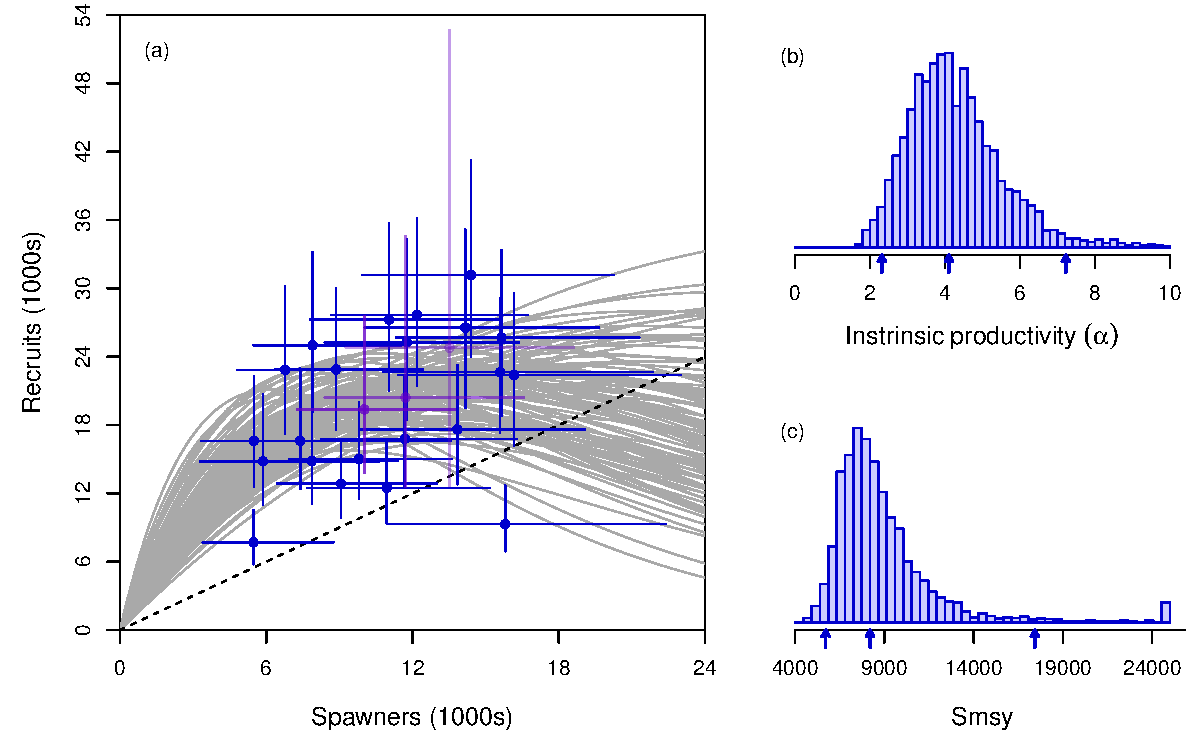
\includegraphics{App_2_Summarize_results_Spring_Chinook_files/figure-latex/plot_S_R-1.pdf}

\begin{Shaded}
\begin{Highlighting}[]
\CommentTok{# ## posterior for K}
\CommentTok{# par(mai=c(0.8,0.4,0.3,0.1))}
\CommentTok{# aa <- matrix(model[,"E_Rkr_a"],ncol=1)}
\CommentTok{# bb <- matrix(model[,"beta"],ncol=1)}
\CommentTok{# R_b_est <- (aa)/bb}
\CommentTok{# R_b_est <- R_b_est[R_b_est > 0]}
\CommentTok{# R_b_CI <- quantile(R_b_est,c(0.025,0.5,0.975))}
\CommentTok{# R_b_est[R_b_est>1.5e4] <- 1.5e4}
\CommentTok{# brks <- seq(Re2prec(min(R_b_est),"floor",2000),1.5e4,length.out=length(seq(0,9,0.2)))}
\CommentTok{# hist(R_b_est, freq=FALSE, breaks=brks, col=clr, border="blue3",}
\CommentTok{#    xlab="", xaxt="n", yaxt="n",}
\CommentTok{#    main="", ylab="", cex.lab=1.2)}
\CommentTok{# axis(1, at=seq(Re2prec(min(R_b_est),"floor",2000),15000,1000))}
\CommentTok{# aHt <- (par()$usr[4]-par()$usr[3])/12}
\CommentTok{# arrows(R_b_CI,par()$usr[3],R_b_CI,par()$usr[3]-aHt,}
\CommentTok{#        code=1,length=0.05,xpd=NA,col="blue3",lwd=1.5)}
\CommentTok{# mtext(expression(Carrying~capacity~(italic(K))), 1, line=3, cex=1)}
\CommentTok{# text(x=par()$usr[1]+par()$pin[2]/par()$pin[1]*offSet*diff(par()$usr[1:2]),}
\CommentTok{#    y=par()$usr[4]-offSet*diff(par()$usr[3:4]),"(c)")}
\end{Highlighting}
\end{Shaded}

\hypertarget{management-reference-points}{%
\subsubsection{Management Reference
Points}\label{management-reference-points}}

Here are a number of management reference points.We make use of the
Lambert W function, W(\emph{z}), which allows for an explicit solution
of Smsy that depends only on parameters \emph{a} and \emph{b} (see
Scheuerell, 2016).

\href{https://peerj.com/articles/1623/}{Scheuerell, M. D. 2016. An
explicit solution for calculating optimum spawning stock size from
Ricker's stock recruitment model. PeerJ, 4: e1623.}

\begin{Shaded}
\begin{Highlighting}[]
\NormalTok{mcmc_samp <-}\StringTok{ }\DecValTok{4000}

\NormalTok{MC <-}\StringTok{ }\DecValTok{100}
\KeywordTok{set.seed}\NormalTok{(}\DecValTok{123}\NormalTok{)}
\NormalTok{idx <-}\StringTok{ }\KeywordTok{sample}\NormalTok{(}\KeywordTok{seq}\NormalTok{(mcmc_samp),MC)}
\CommentTok{# abbreviations for ref points}
\NormalTok{ref_names <-}\StringTok{ }\KeywordTok{c}\NormalTok{(}\StringTok{"MSY"}\NormalTok{,}\StringTok{"Smsy"}\NormalTok{,}\StringTok{"Umsy"}\NormalTok{,}\StringTok{"Umax"}\NormalTok{,}\StringTok{"Seq"}\NormalTok{,}\StringTok{"Scrit"}\NormalTok{)}
\CommentTok{# proportions of MSY to consider}
\NormalTok{yld_prop <-}\StringTok{ }\KeywordTok{c}\NormalTok{(}\FloatTok{0.75}\NormalTok{,}\FloatTok{0.85}\NormalTok{,}\FloatTok{0.95}\NormalTok{)}
\NormalTok{bb <-}\StringTok{ }\NormalTok{model[,}\KeywordTok{grep}\NormalTok{(}\StringTok{"beta"}\NormalTok{,}\KeywordTok{colnames}\NormalTok{(model))]}
\NormalTok{aa <-}\StringTok{ }\KeywordTok{matrix}\NormalTok{(model[,}\StringTok{"E_Rkr_a"}\NormalTok{],}\DataTypeTok{ncol=}\DecValTok{1}\NormalTok{)}
\NormalTok{alpha <-}\StringTok{ }\KeywordTok{matrix}\NormalTok{(model[,}\StringTok{"alpha"}\NormalTok{],}\DataTypeTok{ncol=}\DecValTok{1}\NormalTok{)}
\NormalTok{mcmc <-}\StringTok{ }\KeywordTok{length}\NormalTok{(aa)}
\CommentTok{# empty matrix for ref pts}
\NormalTok{ref.pts <-}\StringTok{ }\KeywordTok{matrix}\NormalTok{(}\OtherTok{NA}\NormalTok{,mcmc,}\KeywordTok{length}\NormalTok{(ref_names))}
\KeywordTok{colnames}\NormalTok{(ref.pts) <-}\StringTok{ }\NormalTok{ref_names}
\CommentTok{# spawner series for optimal yield profile}
\NormalTok{SS <-}\StringTok{ }\KeywordTok{seq}\NormalTok{(}\DecValTok{100}\NormalTok{,}\FloatTok{5e3}\NormalTok{,}\DecValTok{100}\NormalTok{)}
\CommentTok{# empty matrix for optimal yield profiles}
\NormalTok{OYP <-}\StringTok{ }\KeywordTok{matrix}\NormalTok{(}\DecValTok{0}\NormalTok{,}\KeywordTok{length}\NormalTok{(SS),}\KeywordTok{length}\NormalTok{(yld_prop))}
\ControlFlowTok{for}\NormalTok{(i }\ControlFlowTok{in} \DecValTok{1}\OperatorTok{:}\NormalTok{mcmc) \{}
  \CommentTok{# spawners at MSY}
\NormalTok{  ref.pts[i,}\StringTok{"Smsy"}\NormalTok{] <-}\StringTok{ }\NormalTok{(}\DecValTok{1} \OperatorTok{-}\StringTok{ }\KeywordTok{lambert_W0}\NormalTok{(}\KeywordTok{exp}\NormalTok{(}\DecValTok{1}\OperatorTok{-}\NormalTok{aa[i]))) }\OperatorTok{/}\StringTok{ }\NormalTok{bb[i]}
  \CommentTok{# MSY}
\NormalTok{  ref.pts[i,}\StringTok{"MSY"}\NormalTok{] <-}\StringTok{ }\NormalTok{ref.pts[i,}\StringTok{"Smsy"}\NormalTok{]}\OperatorTok{*}\NormalTok{((}\KeywordTok{exp}\NormalTok{(aa[i]}\OperatorTok{-}\NormalTok{bb[i]}\OperatorTok{*}\NormalTok{ref.pts[i,}\StringTok{"Smsy"}\NormalTok{])) }\OperatorTok{-}\StringTok{ }\DecValTok{1}\NormalTok{)}
  \CommentTok{# harvest rate at MSY}
\NormalTok{  ref.pts[i,}\StringTok{"Umsy"}\NormalTok{] <-}\StringTok{ }\NormalTok{(}\DecValTok{1} \OperatorTok{-}\StringTok{ }\KeywordTok{lambert_W0}\NormalTok{(}\KeywordTok{exp}\NormalTok{(}\DecValTok{1}\OperatorTok{-}\NormalTok{aa[i])))}
  \CommentTok{# max harvest rate}
\NormalTok{  ref.pts[i,}\StringTok{"Umax"}\NormalTok{] <-}\StringTok{ }\DecValTok{1} \OperatorTok{-}\StringTok{ }\DecValTok{1}\OperatorTok{/}\NormalTok{alpha[i]}
  \CommentTok{# equilibrium escapement}
\NormalTok{  ref.pts[i,}\StringTok{"Seq"}\NormalTok{] <-}\StringTok{ }\NormalTok{aa[i]}\OperatorTok{/}\NormalTok{bb[i]}
  \CommentTok{# critical escapement}
\NormalTok{  ref.pts[i,}\StringTok{"Scrit"}\NormalTok{] <-}\StringTok{ }\FloatTok{.05}\OperatorTok{*}\NormalTok{ref.pts[i,}\StringTok{"Seq"}\NormalTok{]}
  
  \CommentTok{# yield over varying S}
\NormalTok{  yield <-}\StringTok{ }\NormalTok{SS}\OperatorTok{*}\NormalTok{(}\KeywordTok{exp}\NormalTok{(aa[i]}\OperatorTok{-}\NormalTok{bb[i]}\OperatorTok{*}\NormalTok{SS) }\OperatorTok{-}\StringTok{ }\DecValTok{1}\NormalTok{)}
  \ControlFlowTok{for}\NormalTok{(j }\ControlFlowTok{in} \DecValTok{1}\OperatorTok{:}\KeywordTok{length}\NormalTok{(yld_prop)) \{}
\NormalTok{    OYP[,j] <-}\StringTok{ }\NormalTok{OYP[,j] }\OperatorTok{+}\StringTok{ }\DecValTok{1}\OperatorTok{*}\NormalTok{(yield }\OperatorTok{>}\StringTok{ }\NormalTok{yld_prop[j]}\OperatorTok{*}\NormalTok{ref.pts[i,}\StringTok{"MSY"}\NormalTok{])}
\NormalTok{  \}}
\NormalTok{\}}
\NormalTok{OYP <-}\StringTok{ }\NormalTok{OYP}\OperatorTok{/}\NormalTok{mcmc}


\CommentTok{## Prob of overfishing}
\NormalTok{hh <-}\StringTok{ }\KeywordTok{seq}\NormalTok{(}\DecValTok{100}\NormalTok{)}
\NormalTok{Pr_over <-}\StringTok{ }\KeywordTok{cbind}\NormalTok{(hh,hh,hh)}
\KeywordTok{colnames}\NormalTok{(Pr_over) <-}\StringTok{ }\KeywordTok{c}\NormalTok{(}\StringTok{"Umsy75"}\NormalTok{,}\StringTok{"Umsy"}\NormalTok{,}\StringTok{"Umax"}\NormalTok{)}
\ControlFlowTok{for}\NormalTok{(i }\ControlFlowTok{in}\NormalTok{ hh) \{}
\NormalTok{  Pr_over[i,}\StringTok{"Umsy75"}\NormalTok{] <-}\StringTok{ }\KeywordTok{sum}\NormalTok{(ref.pts[,}\StringTok{"Umsy"}\NormalTok{]}\OperatorTok{*}\FloatTok{0.75} \OperatorTok{<}\StringTok{ }\NormalTok{i}\OperatorTok{/}\DecValTok{100}\NormalTok{)}\OperatorTok{/}\NormalTok{mcmc_samp}
\NormalTok{  Pr_over[i,}\StringTok{"Umsy"}\NormalTok{] <-}\StringTok{ }\KeywordTok{sum}\NormalTok{(ref.pts[,}\StringTok{"Umsy"}\NormalTok{] }\OperatorTok{<}\StringTok{ }\NormalTok{i}\OperatorTok{/}\DecValTok{100}\NormalTok{)}\OperatorTok{/}\NormalTok{mcmc_samp}
\NormalTok{  Pr_over[i,}\StringTok{"Umax"}\NormalTok{] <-}\StringTok{ }\KeywordTok{sum}\NormalTok{(ref.pts[,}\StringTok{"Umax"}\NormalTok{] }\OperatorTok{<}\StringTok{ }\NormalTok{i}\OperatorTok{/}\DecValTok{100}\NormalTok{)}\OperatorTok{/}\NormalTok{mcmc_samp}
\NormalTok{\}}

\CommentTok{## observed exploitation rate & posterior spawner abundance}
\NormalTok{Sp_ts <-}\StringTok{ }\NormalTok{model[,}\KeywordTok{grep}\NormalTok{(}\StringTok{"Sp"}\NormalTok{,}\KeywordTok{colnames}\NormalTok{(model))]}
\end{Highlighting}
\end{Shaded}

These are plots of (a) the probability that a given number of spawners
produce average yields exceeding X\% of MSY (i.e, optimal yield
profiles); and (b) the cumulative probabilty of overfishing the
population, based on harvest rates equal to those at 75\% of MSY
\((U_{\text{M75}})\), MSY \((U_{\text{MSY}})\), and the maximum
\((U_{\text{Max}})\). The probability of exceeding \(U_{\text{Max}}\)
indicates the risk that offspring will not replace their parents, which,
if sustained, will lead to eventual extinction. The histograms above (a)
and (b) are distributions of the posterior estimates for the number of
spawners and harvest rates, respectively

\begin{Shaded}
\begin{Highlighting}[]
\KeywordTok{layout}\NormalTok{(}\KeywordTok{matrix}\NormalTok{(}\KeywordTok{c}\NormalTok{(}\DecValTok{2}\NormalTok{,}\DecValTok{1}\NormalTok{,}\DecValTok{4}\NormalTok{,}\DecValTok{3}\NormalTok{),}\DecValTok{2}\NormalTok{,}\DecValTok{2}\NormalTok{),}\DataTypeTok{heights=}\KeywordTok{c}\NormalTok{(}\DecValTok{1}\NormalTok{,}\DecValTok{5}\NormalTok{))}

\CommentTok{## OYP}
\KeywordTok{par}\NormalTok{(}\DataTypeTok{mai=}\KeywordTok{c}\NormalTok{(}\FloatTok{0.9}\NormalTok{,}\FloatTok{0.9}\NormalTok{,}\DecValTok{0}\NormalTok{,}\DecValTok{0}\NormalTok{), }\DataTypeTok{omi=}\KeywordTok{c}\NormalTok{(}\DecValTok{0}\NormalTok{,}\DecValTok{0}\NormalTok{,}\FloatTok{0.1}\NormalTok{,}\FloatTok{0.1}\NormalTok{))}
\NormalTok{x_lp <-}\StringTok{ }\NormalTok{yld_prop}
\ControlFlowTok{for}\NormalTok{(i }\ControlFlowTok{in} \DecValTok{1}\OperatorTok{:}\KeywordTok{length}\NormalTok{(x_lp)) \{}
\NormalTok{  x_lp[i] <-}\StringTok{ }\NormalTok{SS[}\KeywordTok{max}\NormalTok{(}\KeywordTok{which}\NormalTok{(OYP[,i] }\OperatorTok{==}\StringTok{ }\KeywordTok{max}\NormalTok{(OYP[,i]) }\OperatorTok{|}\StringTok{ }\KeywordTok{abs}\NormalTok{(OYP[,i] }\OperatorTok{-}\StringTok{ }\NormalTok{(yld_prop[i]}\OperatorTok{-}\FloatTok{0.3}\NormalTok{)) }\OperatorTok{<=}\StringTok{ }\FloatTok{0.05}\NormalTok{))]}
\NormalTok{\}}
\KeywordTok{matplot}\NormalTok{(SS, OYP, }\DataTypeTok{type=}\StringTok{"l"}\NormalTok{, }\DataTypeTok{lty=}\StringTok{"solid"}\NormalTok{, }\DataTypeTok{las=}\DecValTok{1}\NormalTok{, }\DataTypeTok{col=}\KeywordTok{c}\NormalTok{(}\StringTok{"slateblue"}\NormalTok{,}\StringTok{"blue"}\NormalTok{,}\StringTok{"darkblue"}\NormalTok{), }\DataTypeTok{lwd=}\DecValTok{2}\NormalTok{,}
        \DataTypeTok{xlab=}\StringTok{"Spawners"}\NormalTok{, }\DataTypeTok{ylab=}\StringTok{"Probability of X% of MSY"}\NormalTok{, }\DataTypeTok{cex.lab=}\FloatTok{1.2}\NormalTok{,}
        \DataTypeTok{main=}\StringTok{""}\NormalTok{, }\DataTypeTok{ylim=}\KeywordTok{c}\NormalTok{(}\DecValTok{0}\NormalTok{,}\DecValTok{1}\NormalTok{))}
\KeywordTok{points}\NormalTok{(}\DataTypeTok{x=}\NormalTok{x_lp, }\DataTypeTok{y=}\NormalTok{yld_prop}\FloatTok{-0.3}\NormalTok{, }\DataTypeTok{pch=}\DecValTok{21}\NormalTok{, }\DataTypeTok{cex=}\FloatTok{3.5}\NormalTok{, }\DataTypeTok{col=}\StringTok{"white"}\NormalTok{, }\DataTypeTok{bg=}\StringTok{"white"}\NormalTok{)}
\KeywordTok{text}\NormalTok{(}\DataTypeTok{x=}\NormalTok{x_lp, }\DataTypeTok{y=}\NormalTok{yld_prop}\FloatTok{-0.3}\NormalTok{, }\KeywordTok{paste0}\NormalTok{(yld_prop}\OperatorTok{*}\DecValTok{100}\NormalTok{,}\StringTok{"%"}\NormalTok{),}
     \DataTypeTok{col=}\KeywordTok{c}\NormalTok{(}\StringTok{"slateblue"}\NormalTok{,}\StringTok{"blue"}\NormalTok{,}\StringTok{"darkblue"}\NormalTok{), }\DataTypeTok{cex=}\FloatTok{0.7}\NormalTok{)}
\KeywordTok{text}\NormalTok{(}\DataTypeTok{x=}\KeywordTok{par}\NormalTok{()}\OperatorTok{$}\NormalTok{usr[}\DecValTok{1}\NormalTok{]}\OperatorTok{+}\KeywordTok{par}\NormalTok{()}\OperatorTok{$}\NormalTok{pin[}\DecValTok{2}\NormalTok{]}\OperatorTok{/}\KeywordTok{par}\NormalTok{()}\OperatorTok{$}\NormalTok{pin[}\DecValTok{1}\NormalTok{]}\OperatorTok{*}\NormalTok{offSet}\OperatorTok{*}\KeywordTok{diff}\NormalTok{(}\KeywordTok{par}\NormalTok{()}\OperatorTok{$}\NormalTok{usr[}\DecValTok{1}\OperatorTok{:}\DecValTok{2}\NormalTok{]),}
     \DataTypeTok{y=}\KeywordTok{par}\NormalTok{()}\OperatorTok{$}\NormalTok{usr[}\DecValTok{4}\NormalTok{]}\OperatorTok{-}\NormalTok{offSet}\OperatorTok{*}\KeywordTok{diff}\NormalTok{(}\KeywordTok{par}\NormalTok{()}\OperatorTok{$}\NormalTok{usr[}\DecValTok{3}\OperatorTok{:}\DecValTok{4}\NormalTok{]),}\StringTok{"(a)"}\NormalTok{)}
\CommentTok{## posterior spawner abundance over all years}
\KeywordTok{par}\NormalTok{(}\DataTypeTok{mai=}\KeywordTok{c}\NormalTok{(}\DecValTok{0}\NormalTok{,}\FloatTok{0.9}\NormalTok{,}\FloatTok{0.05}\NormalTok{,}\DecValTok{0}\NormalTok{))}
\KeywordTok{hist}\NormalTok{(Sp_ts[Sp_ts}\OperatorTok{<}\FloatTok{3e4}\NormalTok{], }\DataTypeTok{col=}\NormalTok{clr, }\DataTypeTok{border=}\StringTok{"blue3"}\NormalTok{, }\DataTypeTok{breaks=}\DecValTok{40}\NormalTok{,}
     \DataTypeTok{main=}\StringTok{""}\NormalTok{, }\DataTypeTok{yaxs=}\StringTok{"i"}\NormalTok{, }\DataTypeTok{xaxt=}\StringTok{"n"}\NormalTok{,}\DataTypeTok{yaxt=}\StringTok{"n"}\NormalTok{,}\DataTypeTok{ylab=}\StringTok{""}\NormalTok{)}

\CommentTok{## prob of overfishing}
\KeywordTok{par}\NormalTok{(}\DataTypeTok{mai=}\KeywordTok{c}\NormalTok{(}\FloatTok{0.9}\NormalTok{,}\FloatTok{0.9}\NormalTok{,}\DecValTok{0}\NormalTok{,}\DecValTok{0}\NormalTok{))}
\KeywordTok{matplot}\NormalTok{(Pr_over, }\DataTypeTok{type=}\StringTok{"l"}\NormalTok{, }\DataTypeTok{las=}\DecValTok{1}\NormalTok{, }\DataTypeTok{lwd=}\DecValTok{2}\NormalTok{, }\DataTypeTok{lty=}\StringTok{"solid"}\NormalTok{, }\DataTypeTok{col=}\KeywordTok{c}\NormalTok{(}\StringTok{"slateblue"}\NormalTok{,}\StringTok{"blue"}\NormalTok{,}\StringTok{"darkblue"}\NormalTok{),}
        \DataTypeTok{ylab=}\StringTok{"Probability of overfishing"}\NormalTok{, }\DataTypeTok{cex.lab=}\FloatTok{1.2}\NormalTok{,}
        \DataTypeTok{xlab=}\StringTok{"Harvest rate"}\NormalTok{, }\DataTypeTok{xaxt=}\StringTok{"n"}\NormalTok{)}
\KeywordTok{axis}\NormalTok{(}\DecValTok{1}\NormalTok{,}\KeywordTok{seq}\NormalTok{(}\DecValTok{0}\NormalTok{,}\DecValTok{100}\NormalTok{,}\DecValTok{20}\NormalTok{),}\KeywordTok{seq}\NormalTok{(}\DecValTok{0}\NormalTok{,}\DecValTok{100}\NormalTok{,}\DecValTok{20}\NormalTok{)}\OperatorTok{/}\DecValTok{100}\NormalTok{)}
\NormalTok{x_lp <-}\StringTok{ }\KeywordTok{c}\NormalTok{(}\DecValTok{0}\NormalTok{,}\DecValTok{0}\NormalTok{,}\DecValTok{0}\NormalTok{)}
\ControlFlowTok{for}\NormalTok{(i }\ControlFlowTok{in} \DecValTok{1}\OperatorTok{:}\KeywordTok{length}\NormalTok{(x_lp)) \{}
\NormalTok{  x_lp[i] <-}\StringTok{ }\KeywordTok{max}\NormalTok{(}\KeywordTok{which}\NormalTok{(}\KeywordTok{abs}\NormalTok{(Pr_over[,i] }\OperatorTok{-}\StringTok{ }\FloatTok{0.5}\NormalTok{) }\OperatorTok{<=}\StringTok{ }\FloatTok{0.05}\NormalTok{))}
\NormalTok{\}}
\KeywordTok{points}\NormalTok{(}\DataTypeTok{x=}\NormalTok{x_lp, }\DataTypeTok{y=}\KeywordTok{rep}\NormalTok{(}\FloatTok{0.5}\NormalTok{,}\DecValTok{3}\NormalTok{), }\DataTypeTok{pch=}\DecValTok{21}\NormalTok{, }\DataTypeTok{cex=}\DecValTok{4}\NormalTok{, }\DataTypeTok{col=}\StringTok{"white"}\NormalTok{, }\DataTypeTok{bg=}\StringTok{"white"}\NormalTok{)}
\KeywordTok{text}\NormalTok{(}\DataTypeTok{x=}\NormalTok{x_lp, }\DataTypeTok{y=}\FloatTok{0.5}\NormalTok{, }\KeywordTok{expression}\NormalTok{(U[M75], U[MSY], U[Max]),}
     \DataTypeTok{col=}\KeywordTok{c}\NormalTok{(}\StringTok{"slateblue"}\NormalTok{,}\StringTok{"blue"}\NormalTok{,}\StringTok{"darkblue"}\NormalTok{), }\DataTypeTok{cex=}\FloatTok{0.8}\NormalTok{)}
\KeywordTok{text}\NormalTok{(}\DataTypeTok{x=}\KeywordTok{par}\NormalTok{()}\OperatorTok{$}\NormalTok{usr[}\DecValTok{1}\NormalTok{]}\OperatorTok{+}\KeywordTok{par}\NormalTok{()}\OperatorTok{$}\NormalTok{pin[}\DecValTok{2}\NormalTok{]}\OperatorTok{/}\KeywordTok{par}\NormalTok{()}\OperatorTok{$}\NormalTok{pin[}\DecValTok{1}\NormalTok{]}\OperatorTok{*}\NormalTok{offSet}\OperatorTok{*}\KeywordTok{diff}\NormalTok{(}\KeywordTok{par}\NormalTok{()}\OperatorTok{$}\NormalTok{usr[}\DecValTok{1}\OperatorTok{:}\DecValTok{2}\NormalTok{]),}
     \DataTypeTok{y=}\KeywordTok{par}\NormalTok{()}\OperatorTok{$}\NormalTok{usr[}\DecValTok{4}\NormalTok{]}\OperatorTok{-}\NormalTok{offSet}\OperatorTok{*}\KeywordTok{diff}\NormalTok{(}\KeywordTok{par}\NormalTok{()}\OperatorTok{$}\NormalTok{usr[}\DecValTok{3}\OperatorTok{:}\DecValTok{4}\NormalTok{]),}\StringTok{"(b)"}\NormalTok{)}
\end{Highlighting}
\end{Shaded}

\includegraphics{App_2_Summarize_results_Spring_Chinook_files/figure-latex/plot_ref_pts-1.pdf}

Here is a summary of estimated reference points

\begin{Shaded}
\begin{Highlighting}[]
\NormalTok{tbl_refpt_smry <-}\StringTok{ }\KeywordTok{apply}\NormalTok{(ref.pts,}\DecValTok{2}\NormalTok{,quantile,CI_vec)}
\KeywordTok{print}\NormalTok{(tbl_refpt_smry,}\DataTypeTok{digits=}\DecValTok{3}\NormalTok{,}\DataTypeTok{quote=}\OtherTok{FALSE}\NormalTok{,}\DataTypeTok{justify=}\StringTok{"right"}\NormalTok{)}
\end{Highlighting}
\end{Shaded}

\begin{verbatim}
##        MSY Smsy  Umsy  Umax   Seq Scrit
## 2.5%   496  576 0.233 0.314  1534  76.7
## 50%    960 1024 0.452 0.597  2403 120.2
## 97.5% 2828 6987 0.726 0.839 15042 752.1
\end{verbatim}

\hypertarget{total-population-size}{%
\subsubsection{Total population size}\label{total-population-size}}

Here is our estimate of the escapement over time through return year
2014. The black points are the data, the blue line is the median
posterior estimate, and the shaded region is the 95\% credible interval.
Note that the y-axis is on a log scale.

\begin{Shaded}
\begin{Highlighting}[]
\NormalTok{pDat <-}\StringTok{ }\KeywordTok{apply}\NormalTok{(model[,}\KeywordTok{grep}\NormalTok{(}\StringTok{"Sp"}\NormalTok{,}\KeywordTok{colnames}\NormalTok{(model))],}\DecValTok{2}\NormalTok{,quantile,CI_vec)}

\NormalTok{ypMin <-}\StringTok{ }\KeywordTok{min}\NormalTok{(pDat[,}\DecValTok{1}\OperatorTok{:}\NormalTok{n_yrs])}
\NormalTok{ypMax <-}\StringTok{ }\KeywordTok{max}\NormalTok{(pDat[,}\DecValTok{1}\OperatorTok{:}\NormalTok{n_yrs])}
\NormalTok{t_idx_T <-}\StringTok{ }\KeywordTok{seq}\NormalTok{(yr_frst,}\DataTypeTok{length.out=}\NormalTok{n_yrs)}
\KeywordTok{par}\NormalTok{(}\DataTypeTok{mai=}\KeywordTok{c}\NormalTok{(}\FloatTok{0.8}\NormalTok{,}\FloatTok{0.8}\NormalTok{,}\FloatTok{0.1}\NormalTok{,}\FloatTok{0.1}\NormalTok{), }\DataTypeTok{omi=}\KeywordTok{c}\NormalTok{(}\DecValTok{0}\NormalTok{,}\FloatTok{0.2}\NormalTok{,}\FloatTok{0.1}\NormalTok{,}\FloatTok{0.2}\NormalTok{))}
\KeywordTok{plot}\NormalTok{(t_idx_T,pDat[}\DecValTok{3}\NormalTok{,}\DecValTok{1}\OperatorTok{:}\NormalTok{n_yrs], }\DataTypeTok{ylim=}\KeywordTok{c}\NormalTok{(ypMin,ypMax), }\DataTypeTok{type=}\StringTok{"n"}\NormalTok{, }\DataTypeTok{log=}\StringTok{"y"}\NormalTok{, }\DataTypeTok{xaxt=}\StringTok{"n"}\NormalTok{, }\DataTypeTok{yaxt=}\StringTok{"n"}\NormalTok{,}
     \DataTypeTok{xlab=}\StringTok{"Year"}\NormalTok{, }\DataTypeTok{ylab=}\StringTok{"Spawners"}\NormalTok{, }\DataTypeTok{main=}\StringTok{""}\NormalTok{, }\DataTypeTok{cex.lab=}\FloatTok{1.2}\NormalTok{)}
\KeywordTok{polygon}\NormalTok{(}\KeywordTok{c}\NormalTok{(t_idx_T,}\KeywordTok{rev}\NormalTok{(t_idx_T)),}\KeywordTok{c}\NormalTok{(pDat[}\DecValTok{3}\NormalTok{,}\DecValTok{1}\OperatorTok{:}\NormalTok{n_yrs],}\KeywordTok{rev}\NormalTok{(pDat[}\DecValTok{1}\NormalTok{,}\DecValTok{1}\OperatorTok{:}\NormalTok{n_yrs])), }\DataTypeTok{col=}\NormalTok{clr, }\DataTypeTok{border=}\OtherTok{NA}\NormalTok{)}
\KeywordTok{lines}\NormalTok{(t_idx_T, pDat[}\DecValTok{2}\NormalTok{,}\DecValTok{1}\OperatorTok{:}\NormalTok{n_yrs], }\DataTypeTok{col=}\StringTok{"blue3"}\NormalTok{, }\DataTypeTok{lwd=}\DecValTok{2}\NormalTok{)}
\KeywordTok{points}\NormalTok{(}\KeywordTok{seq}\NormalTok{(yr_frst,}\DataTypeTok{length.out=}\NormalTok{n_yrs), }\KeywordTok{exp}\NormalTok{(ln_dat_esc), }\DataTypeTok{pch=}\DecValTok{16}\NormalTok{, }\DataTypeTok{cex=}\DecValTok{1}\NormalTok{)}
\KeywordTok{axis}\NormalTok{(}\DecValTok{1}\NormalTok{,}\DataTypeTok{at=}\KeywordTok{seq}\NormalTok{(}\DecValTok{1986}\NormalTok{,}\DecValTok{2015}\NormalTok{,}\DecValTok{5}\NormalTok{))}
\KeywordTok{axis}\NormalTok{(}\DecValTok{2}\NormalTok{,}\DataTypeTok{at=}\KeywordTok{c}\NormalTok{(}\DecValTok{500}\NormalTok{,}\DecValTok{1000}\NormalTok{,}\DecValTok{3000}\NormalTok{))}
\end{Highlighting}
\end{Shaded}

\includegraphics{App_2_Summarize_results_Spring_Chinook_files/figure-latex/plot_escapement-1.pdf}

\hypertarget{innovations}{%
\subsubsection{Innovations}\label{innovations}}

Here is the time series of the so-called ``innovations'', which are the
residuals from the process model. They give some indication of
population productivity after accounting for the effects of density
dependence.

\begin{Shaded}
\begin{Highlighting}[]
\NormalTok{t_idx_a <-}\StringTok{ }\KeywordTok{seq}\NormalTok{(yr_frst,}\DataTypeTok{length.out=}\NormalTok{n_yrs}\OperatorTok{-}\NormalTok{age_min)}
\CommentTok{#pDat <- apply(mod_fit$BUGSoutput$sims.list$res_ln_Rec,2,quantile,CI_vec)}
\NormalTok{pDat <-}\StringTok{ }\KeywordTok{apply}\NormalTok{(model[,}\KeywordTok{grep}\NormalTok{(}\StringTok{"res_ln_Rec"}\NormalTok{,}\KeywordTok{colnames}\NormalTok{(model))],}\DecValTok{2}\NormalTok{,quantile,CI_vec)}
\NormalTok{ypMin <-}\StringTok{ }\KeywordTok{min}\NormalTok{(pDat)}
\NormalTok{ypMax <-}\StringTok{ }\KeywordTok{max}\NormalTok{(pDat)}
\KeywordTok{par}\NormalTok{(}\DataTypeTok{mai=}\KeywordTok{c}\NormalTok{(}\FloatTok{0.8}\NormalTok{,}\FloatTok{0.8}\NormalTok{,}\FloatTok{0.1}\NormalTok{,}\FloatTok{0.1}\NormalTok{), }\DataTypeTok{omi=}\KeywordTok{c}\NormalTok{(}\DecValTok{0}\NormalTok{,}\FloatTok{0.2}\NormalTok{,}\FloatTok{0.1}\NormalTok{,}\FloatTok{0.2}\NormalTok{))}
\KeywordTok{plot}\NormalTok{(t_idx_a,pDat[}\DecValTok{3}\NormalTok{,], }\DataTypeTok{ylim=}\KeywordTok{c}\NormalTok{(ypMin,ypMax), }\DataTypeTok{type=}\StringTok{"n"}\NormalTok{, }\CommentTok{#log="y",}
     \DataTypeTok{xlab=}\StringTok{"Brood year"}\NormalTok{, }\DataTypeTok{ylab=}\StringTok{"Innovations"}\NormalTok{, }\DataTypeTok{main=}\StringTok{""}\NormalTok{, }\DataTypeTok{cex.lab=}\FloatTok{1.2}\NormalTok{)}
\KeywordTok{abline}\NormalTok{(}\DataTypeTok{h=}\DecValTok{0}\NormalTok{, }\DataTypeTok{lty=}\StringTok{"dashed"}\NormalTok{)}
\KeywordTok{polygon}\NormalTok{(}\KeywordTok{c}\NormalTok{(t_idx_a,}\KeywordTok{rev}\NormalTok{(t_idx_a)),}\KeywordTok{c}\NormalTok{(pDat[}\DecValTok{3}\NormalTok{,],}\KeywordTok{rev}\NormalTok{(pDat[}\DecValTok{1}\NormalTok{,])), }\DataTypeTok{col=}\NormalTok{clr, }\DataTypeTok{border=}\OtherTok{NA}\NormalTok{)}
\KeywordTok{lines}\NormalTok{(t_idx_a, pDat[}\DecValTok{2}\NormalTok{,], }\DataTypeTok{col=}\StringTok{"blue3"}\NormalTok{, }\DataTypeTok{lwd=}\DecValTok{2}\NormalTok{)}
\end{Highlighting}
\end{Shaded}

\includegraphics{App_2_Summarize_results_Spring_Chinook_files/figure-latex/plot_innovations-1.pdf}

\hypertarget{recruitment}{%
\subsubsection{Recruitment}\label{recruitment}}

Here is the posterior time series total annual adult recruitment
produced from each spawning cohort.

\begin{Shaded}
\begin{Highlighting}[]
\NormalTok{t_idx_a <-}\StringTok{ }\KeywordTok{seq}\NormalTok{(yr_frst,}\DataTypeTok{length.out=}\NormalTok{n_yrs}\OperatorTok{-}\NormalTok{age_min)}
\CommentTok{#pDat <- apply(mod_fit$BUGSoutput$sims.list$res_ln_Rec,2,quantile,CI_vec)}
\NormalTok{pDat <-}\StringTok{ }\KeywordTok{exp}\NormalTok{(}\KeywordTok{apply}\NormalTok{(model[,}\KeywordTok{grep}\NormalTok{(}\StringTok{"tot_ln_Rec"}\NormalTok{,}\KeywordTok{colnames}\NormalTok{(model))],}\DecValTok{2}\NormalTok{,quantile,CI_vec))}
\NormalTok{ypMin <-}\StringTok{ }\KeywordTok{min}\NormalTok{(pDat)}
\NormalTok{ypMax <-}\StringTok{ }\KeywordTok{max}\NormalTok{(pDat)}\OperatorTok{+}\DecValTok{1000}
\KeywordTok{par}\NormalTok{(}\DataTypeTok{mai=}\KeywordTok{c}\NormalTok{(}\FloatTok{0.8}\NormalTok{,}\FloatTok{0.8}\NormalTok{,}\FloatTok{0.1}\NormalTok{,}\FloatTok{0.1}\NormalTok{), }\DataTypeTok{omi=}\KeywordTok{c}\NormalTok{(}\DecValTok{0}\NormalTok{,}\FloatTok{0.2}\NormalTok{,}\FloatTok{0.1}\NormalTok{,}\FloatTok{0.2}\NormalTok{))}
\KeywordTok{plot}\NormalTok{(t_idx_a,pDat[}\DecValTok{3}\NormalTok{,], }\DataTypeTok{ylim=}\KeywordTok{c}\NormalTok{(ypMin,ypMax), }\DataTypeTok{type=}\StringTok{"n"}\NormalTok{, }\DataTypeTok{log=}\StringTok{"y"}\NormalTok{,}
     \DataTypeTok{xlab=}\StringTok{"Brood year"}\NormalTok{, }\DataTypeTok{ylab=}\StringTok{"Total Adult Recruitment"}\NormalTok{, }\DataTypeTok{main=}\StringTok{""}\NormalTok{, }\DataTypeTok{cex.lab=}\FloatTok{1.2}\NormalTok{)}
\KeywordTok{abline}\NormalTok{(}\DataTypeTok{h=}\DecValTok{0}\NormalTok{, }\DataTypeTok{lty=}\StringTok{"dashed"}\NormalTok{)}
\KeywordTok{polygon}\NormalTok{(}\KeywordTok{c}\NormalTok{(t_idx_a,}\KeywordTok{rev}\NormalTok{(t_idx_a)),}\KeywordTok{c}\NormalTok{(pDat[}\DecValTok{3}\NormalTok{,],}\KeywordTok{rev}\NormalTok{(pDat[}\DecValTok{1}\NormalTok{,])), }\DataTypeTok{col=}\NormalTok{clr, }\DataTypeTok{border=}\OtherTok{NA}\NormalTok{)}
\KeywordTok{lines}\NormalTok{(t_idx_a, pDat[}\DecValTok{2}\NormalTok{,], }\DataTypeTok{col=}\StringTok{"blue3"}\NormalTok{, }\DataTypeTok{lwd=}\DecValTok{2}\NormalTok{)}
\end{Highlighting}
\end{Shaded}

\includegraphics{App_2_Summarize_results_Spring_Chinook_files/figure-latex/plot_recruitment-1.pdf}

\hypertarget{escapement-recruitment-innovations}{%
\subsubsection{Escapement, Recruitment,
Innovations}\label{escapement-recruitment-innovations}}

\begin{Shaded}
\begin{Highlighting}[]
\KeywordTok{layout}\NormalTok{(}\KeywordTok{matrix}\NormalTok{(}\KeywordTok{c}\NormalTok{(}\DecValTok{1}\NormalTok{,}\DecValTok{2}\NormalTok{,}\DecValTok{3}\NormalTok{,}\DecValTok{4}\NormalTok{),}\DecValTok{2}\NormalTok{,}\DecValTok{2}\NormalTok{),}\KeywordTok{c}\NormalTok{(}\DecValTok{3}\NormalTok{,}\DecValTok{3}\NormalTok{),}\KeywordTok{c}\NormalTok{(}\DecValTok{3}\NormalTok{,}\DecValTok{3}\NormalTok{))}


\NormalTok{offSet <-}\StringTok{ }\FloatTok{0.06}



\NormalTok{pDat <-}\StringTok{ }\KeywordTok{apply}\NormalTok{(model[,}\KeywordTok{grep}\NormalTok{(}\StringTok{"Sp"}\NormalTok{,}\KeywordTok{colnames}\NormalTok{(model))],}\DecValTok{2}\NormalTok{,quantile,CI_vec)}

\CommentTok{##Escapement}
\NormalTok{ypMin <-}\StringTok{ }\KeywordTok{min}\NormalTok{(pDat[,}\DecValTok{1}\OperatorTok{:}\NormalTok{n_yrs])}
\NormalTok{ypMax <-}\StringTok{ }\KeywordTok{max}\NormalTok{(pDat[,}\DecValTok{1}\OperatorTok{:}\NormalTok{n_yrs])}
\NormalTok{t_idx_T <-}\StringTok{ }\KeywordTok{seq}\NormalTok{(yr_frst,}\DataTypeTok{length.out=}\NormalTok{n_yrs)}

\KeywordTok{par}\NormalTok{(}\DataTypeTok{mai=}\KeywordTok{c}\NormalTok{(}\FloatTok{0.8}\NormalTok{,}\FloatTok{0.8}\NormalTok{,}\FloatTok{0.1}\NormalTok{,}\FloatTok{0.1}\NormalTok{), }\DataTypeTok{omi=}\KeywordTok{c}\NormalTok{(}\FloatTok{0.2}\NormalTok{,}\DecValTok{0}\NormalTok{,}\DecValTok{0}\NormalTok{,}\DecValTok{0}\NormalTok{))}
\CommentTok{#par(mai=c(0.8,0.8,0.1,0.1), omi=c(0,0.2,0.1,0.2))}

\KeywordTok{plot}\NormalTok{(t_idx_T,pDat[}\DecValTok{3}\NormalTok{,}\DecValTok{1}\OperatorTok{:}\NormalTok{n_yrs], }\DataTypeTok{ylim=}\KeywordTok{c}\NormalTok{(ypMin,ypMax), }\DataTypeTok{type=}\StringTok{"n"}\NormalTok{, }\DataTypeTok{log=}\StringTok{"y"}\NormalTok{, }
     \DataTypeTok{xaxt=}\StringTok{"n"}\NormalTok{, }\DataTypeTok{yaxt=}\StringTok{"n"}\NormalTok{,}
     \DataTypeTok{xlab=}\StringTok{"Year"}\NormalTok{, }\DataTypeTok{ylab=}\StringTok{"Spawners"}\NormalTok{, }\DataTypeTok{main=}\StringTok{""}\NormalTok{, }\DataTypeTok{cex.lab=}\FloatTok{1.2}\NormalTok{)}
\KeywordTok{polygon}\NormalTok{(}\KeywordTok{c}\NormalTok{(t_idx_T,}\KeywordTok{rev}\NormalTok{(t_idx_T)),}\KeywordTok{c}\NormalTok{(pDat[}\DecValTok{3}\NormalTok{,}\DecValTok{1}\OperatorTok{:}\NormalTok{n_yrs],}\KeywordTok{rev}\NormalTok{(pDat[}\DecValTok{1}\NormalTok{,}\DecValTok{1}\OperatorTok{:}\NormalTok{n_yrs])), }\DataTypeTok{col=}\NormalTok{clr, }\DataTypeTok{border=}\OtherTok{NA}\NormalTok{)}
\KeywordTok{lines}\NormalTok{(t_idx_T, pDat[}\DecValTok{2}\NormalTok{,}\DecValTok{1}\OperatorTok{:}\NormalTok{n_yrs], }\DataTypeTok{col=}\StringTok{"blue3"}\NormalTok{, }\DataTypeTok{lwd=}\DecValTok{2}\NormalTok{)}
\KeywordTok{points}\NormalTok{(}\KeywordTok{seq}\NormalTok{(yr_frst,}\DataTypeTok{length.out=}\NormalTok{n_yrs), }\KeywordTok{exp}\NormalTok{(ln_dat_esc), }\DataTypeTok{pch=}\DecValTok{16}\NormalTok{, }\DataTypeTok{cex=}\DecValTok{1}\NormalTok{)}
\KeywordTok{axis}\NormalTok{(}\DecValTok{1}\NormalTok{,}\DataTypeTok{at=}\KeywordTok{seq}\NormalTok{(}\DecValTok{1980}\NormalTok{,}\DecValTok{2015}\NormalTok{,}\DecValTok{5}\NormalTok{))}
\KeywordTok{axis}\NormalTok{(}\DecValTok{2}\NormalTok{,}\DataTypeTok{at=}\KeywordTok{c}\NormalTok{(}\DecValTok{500}\NormalTok{,}\DecValTok{1000}\NormalTok{,}\DecValTok{3000}\NormalTok{))}
\KeywordTok{text}\NormalTok{(}\DataTypeTok{x=}\KeywordTok{par}\NormalTok{()}\OperatorTok{$}\NormalTok{usr[}\DecValTok{1}\NormalTok{]}\OperatorTok{+}\KeywordTok{par}\NormalTok{()}\OperatorTok{$}\NormalTok{pin[}\DecValTok{2}\NormalTok{]}\OperatorTok{/}\KeywordTok{par}\NormalTok{()}\OperatorTok{$}\NormalTok{pin[}\DecValTok{1}\NormalTok{]}\OperatorTok{*}\NormalTok{offSet}\OperatorTok{*}\KeywordTok{diff}\NormalTok{(}\KeywordTok{par}\NormalTok{()}\OperatorTok{$}\NormalTok{usr[}\DecValTok{1}\OperatorTok{:}\DecValTok{2}\NormalTok{]),}
     \DataTypeTok{y=}\DecValTok{10}\OperatorTok{^}\KeywordTok{par}\NormalTok{()}\OperatorTok{$}\NormalTok{usr[}\DecValTok{4}\NormalTok{]}\OperatorTok{-}\FloatTok{0.14}\OperatorTok{*}\KeywordTok{diff}\NormalTok{(}\DecValTok{10}\OperatorTok{^}\KeywordTok{par}\NormalTok{()}\OperatorTok{$}\NormalTok{usr[}\DecValTok{3}\OperatorTok{:}\DecValTok{4}\NormalTok{]),}\StringTok{"(a)"}\NormalTok{)}

\CommentTok{##Recruitment}
\NormalTok{t_idx_a <-}\StringTok{ }\KeywordTok{seq}\NormalTok{(yr_frst,}\DataTypeTok{length.out=}\NormalTok{n_yrs}\OperatorTok{-}\NormalTok{age_min)}
\CommentTok{#pDat <- apply(mod_fit$BUGSoutput$sims.list$res_ln_Rec,2,quantile,CI_vec)}
\NormalTok{pDat <-}\StringTok{ }\KeywordTok{exp}\NormalTok{(}\KeywordTok{apply}\NormalTok{(model[,}\KeywordTok{grep}\NormalTok{(}\StringTok{"tot_ln_Rec"}\NormalTok{,}\KeywordTok{colnames}\NormalTok{(model))],}\DecValTok{2}\NormalTok{,quantile,CI_vec))}
\NormalTok{ypMin <-}\StringTok{ }\KeywordTok{min}\NormalTok{(pDat)}
\NormalTok{ypMax <-}\StringTok{ }\KeywordTok{max}\NormalTok{(pDat)}\OperatorTok{+}\DecValTok{1000}
\CommentTok{#par(mai=c(0.8,0.8,0.1,0.1), omi=c(0,0.2,0.1,0.2))}
\KeywordTok{par}\NormalTok{(}\DataTypeTok{mai=}\KeywordTok{c}\NormalTok{(}\FloatTok{0.8}\NormalTok{,}\FloatTok{0.8}\NormalTok{,}\FloatTok{0.1}\NormalTok{,}\FloatTok{0.1}\NormalTok{))}
\KeywordTok{plot}\NormalTok{(t_idx_a,pDat[}\DecValTok{3}\NormalTok{,], }\DataTypeTok{ylim=}\KeywordTok{c}\NormalTok{(ypMin,ypMax), }\DataTypeTok{type=}\StringTok{"n"}\NormalTok{, }\DataTypeTok{log=}\StringTok{"y"}\NormalTok{,}
     \DataTypeTok{xlab=}\StringTok{"Brood year"}\NormalTok{, }\DataTypeTok{ylab=}\StringTok{"Total Adult Recruitment"}\NormalTok{, }\DataTypeTok{main=}\StringTok{""}\NormalTok{, }\DataTypeTok{cex.lab=}\FloatTok{1.2}\NormalTok{)}
\KeywordTok{abline}\NormalTok{(}\DataTypeTok{h=}\DecValTok{0}\NormalTok{, }\DataTypeTok{lty=}\StringTok{"dashed"}\NormalTok{)}
\KeywordTok{polygon}\NormalTok{(}\KeywordTok{c}\NormalTok{(t_idx_a,}\KeywordTok{rev}\NormalTok{(t_idx_a)),}\KeywordTok{c}\NormalTok{(pDat[}\DecValTok{3}\NormalTok{,],}\KeywordTok{rev}\NormalTok{(pDat[}\DecValTok{1}\NormalTok{,])), }\DataTypeTok{col=}\NormalTok{clr, }\DataTypeTok{border=}\OtherTok{NA}\NormalTok{)}
\KeywordTok{lines}\NormalTok{(t_idx_a, pDat[}\DecValTok{2}\NormalTok{,], }\DataTypeTok{col=}\StringTok{"blue3"}\NormalTok{, }\DataTypeTok{lwd=}\DecValTok{2}\NormalTok{)}
\KeywordTok{text}\NormalTok{(}\DataTypeTok{x=}\KeywordTok{par}\NormalTok{()}\OperatorTok{$}\NormalTok{usr[}\DecValTok{1}\NormalTok{]}\OperatorTok{+}\KeywordTok{par}\NormalTok{()}\OperatorTok{$}\NormalTok{pin[}\DecValTok{2}\NormalTok{]}\OperatorTok{/}\KeywordTok{par}\NormalTok{()}\OperatorTok{$}\NormalTok{pin[}\DecValTok{1}\NormalTok{]}\OperatorTok{*}\NormalTok{offSet}\OperatorTok{*}\KeywordTok{diff}\NormalTok{(}\KeywordTok{par}\NormalTok{()}\OperatorTok{$}\NormalTok{usr[}\DecValTok{1}\OperatorTok{:}\DecValTok{2}\NormalTok{]),}
     \DataTypeTok{y=}\DecValTok{10}\OperatorTok{^}\KeywordTok{par}\NormalTok{()}\OperatorTok{$}\NormalTok{usr[}\DecValTok{4}\NormalTok{]}\OperatorTok{-}\FloatTok{0.14}\OperatorTok{*}\KeywordTok{diff}\NormalTok{(}\DecValTok{10}\OperatorTok{^}\KeywordTok{par}\NormalTok{()}\OperatorTok{$}\NormalTok{usr[}\DecValTok{3}\OperatorTok{:}\DecValTok{4}\NormalTok{]),}\StringTok{"(b)"}\NormalTok{)}
\CommentTok{##Innovations}
\NormalTok{t_idx_a <-}\StringTok{ }\KeywordTok{seq}\NormalTok{(yr_frst,}\DataTypeTok{length.out=}\NormalTok{n_yrs}\OperatorTok{-}\NormalTok{age_min)}
\CommentTok{#pDat <- apply(mod_fit$BUGSoutput$sims.list$res_ln_Rec,2,quantile,CI_vec)}
\NormalTok{pDat <-}\StringTok{ }\KeywordTok{apply}\NormalTok{(model[,}\KeywordTok{grep}\NormalTok{(}\StringTok{"ln_RS"}\NormalTok{,}\KeywordTok{colnames}\NormalTok{(model))],}\DecValTok{2}\NormalTok{,quantile,CI_vec)}
\NormalTok{ypMin <-}\StringTok{ }\KeywordTok{min}\NormalTok{(pDat)}
\NormalTok{ypMax <-}\StringTok{ }\KeywordTok{max}\NormalTok{(pDat)}
\CommentTok{#par(mai=c(0.8,0.8,0.1,0.1), omi=c(0,0.2,0.1,0.2))}
\KeywordTok{par}\NormalTok{(}\DataTypeTok{mai=}\KeywordTok{c}\NormalTok{(}\FloatTok{0.8}\NormalTok{,}\FloatTok{0.8}\NormalTok{,}\FloatTok{0.1}\NormalTok{,}\FloatTok{0.1}\NormalTok{))}
\KeywordTok{plot}\NormalTok{(t_idx_a,pDat[}\DecValTok{3}\NormalTok{,], }\DataTypeTok{ylim=}\KeywordTok{c}\NormalTok{(ypMin,ypMax), }\DataTypeTok{type=}\StringTok{"n"}\NormalTok{,}
     \DataTypeTok{xlab=}\StringTok{"Brood year"}\NormalTok{, }\DataTypeTok{ylab=}\StringTok{"ln(R/S)"}\NormalTok{, }\DataTypeTok{main=}\StringTok{""}\NormalTok{, }\DataTypeTok{cex.lab=}\FloatTok{1.2}\NormalTok{)}
\KeywordTok{abline}\NormalTok{(}\DataTypeTok{h=}\DecValTok{0}\NormalTok{, }\DataTypeTok{lty=}\StringTok{"dashed"}\NormalTok{)}
\KeywordTok{polygon}\NormalTok{(}\KeywordTok{c}\NormalTok{(t_idx_a,}\KeywordTok{rev}\NormalTok{(t_idx_a)),}\KeywordTok{c}\NormalTok{(pDat[}\DecValTok{3}\NormalTok{,],}\KeywordTok{rev}\NormalTok{(pDat[}\DecValTok{1}\NormalTok{,])), }\DataTypeTok{col=}\NormalTok{clr, }\DataTypeTok{border=}\OtherTok{NA}\NormalTok{)}
\KeywordTok{lines}\NormalTok{(t_idx_a, pDat[}\DecValTok{2}\NormalTok{,], }\DataTypeTok{col=}\StringTok{"blue3"}\NormalTok{, }\DataTypeTok{lwd=}\DecValTok{2}\NormalTok{)}
\KeywordTok{text}\NormalTok{(}\DataTypeTok{x=}\KeywordTok{par}\NormalTok{()}\OperatorTok{$}\NormalTok{usr[}\DecValTok{1}\NormalTok{]}\OperatorTok{+}\KeywordTok{par}\NormalTok{()}\OperatorTok{$}\NormalTok{pin[}\DecValTok{2}\NormalTok{]}\OperatorTok{/}\KeywordTok{par}\NormalTok{()}\OperatorTok{$}\NormalTok{pin[}\DecValTok{1}\NormalTok{]}\OperatorTok{*}\NormalTok{offSet}\OperatorTok{*}\KeywordTok{diff}\NormalTok{(}\KeywordTok{par}\NormalTok{()}\OperatorTok{$}\NormalTok{usr[}\DecValTok{1}\OperatorTok{:}\DecValTok{2}\NormalTok{]),}
     \DataTypeTok{y=}\KeywordTok{par}\NormalTok{()}\OperatorTok{$}\NormalTok{usr[}\DecValTok{4}\NormalTok{]}\OperatorTok{-}\NormalTok{offSet}\OperatorTok{*}\KeywordTok{diff}\NormalTok{(}\KeywordTok{par}\NormalTok{()}\OperatorTok{$}\NormalTok{usr[}\DecValTok{3}\OperatorTok{:}\DecValTok{4}\NormalTok{]),}\StringTok{"(c)"}\NormalTok{)}

\CommentTok{##Innovations}
\NormalTok{t_idx_a <-}\StringTok{ }\KeywordTok{seq}\NormalTok{(yr_frst,}\DataTypeTok{length.out=}\NormalTok{n_yrs}\OperatorTok{-}\NormalTok{age_min)}
\CommentTok{#pDat <- apply(mod_fit$BUGSoutput$sims.list$res_ln_Rec,2,quantile,CI_vec)}
\NormalTok{pDat <-}\StringTok{ }\KeywordTok{apply}\NormalTok{(model[,}\KeywordTok{grep}\NormalTok{(}\StringTok{"res_ln_Rec"}\NormalTok{,}\KeywordTok{colnames}\NormalTok{(model))],}\DecValTok{2}\NormalTok{,quantile,CI_vec)}
\NormalTok{ypMin <-}\StringTok{ }\KeywordTok{min}\NormalTok{(pDat)}
\NormalTok{ypMax <-}\StringTok{ }\KeywordTok{max}\NormalTok{(pDat)}
\CommentTok{#par(mai=c(0.8,0.8,0.1,0.1), omi=c(0,0.2,0.1,0.2))}
\KeywordTok{par}\NormalTok{(}\DataTypeTok{mai=}\KeywordTok{c}\NormalTok{(}\FloatTok{0.8}\NormalTok{,}\FloatTok{0.8}\NormalTok{,}\FloatTok{0.1}\NormalTok{,}\FloatTok{0.1}\NormalTok{))}
\KeywordTok{plot}\NormalTok{(t_idx_a,pDat[}\DecValTok{3}\NormalTok{,], }\DataTypeTok{ylim=}\KeywordTok{c}\NormalTok{(ypMin,ypMax), }\DataTypeTok{type=}\StringTok{"n"}\NormalTok{,}
     \DataTypeTok{xlab=}\StringTok{"Brood year"}\NormalTok{, }\DataTypeTok{ylab=}\StringTok{"Recruitment Residuals"}\NormalTok{, }\DataTypeTok{main=}\StringTok{""}\NormalTok{, }\DataTypeTok{cex.lab=}\FloatTok{1.2}\NormalTok{)}
\KeywordTok{abline}\NormalTok{(}\DataTypeTok{h=}\DecValTok{0}\NormalTok{, }\DataTypeTok{lty=}\StringTok{"dashed"}\NormalTok{)}
\KeywordTok{polygon}\NormalTok{(}\KeywordTok{c}\NormalTok{(t_idx_a,}\KeywordTok{rev}\NormalTok{(t_idx_a)),}\KeywordTok{c}\NormalTok{(pDat[}\DecValTok{3}\NormalTok{,],}\KeywordTok{rev}\NormalTok{(pDat[}\DecValTok{1}\NormalTok{,])), }\DataTypeTok{col=}\NormalTok{clr, }\DataTypeTok{border=}\OtherTok{NA}\NormalTok{)}
\KeywordTok{lines}\NormalTok{(t_idx_a, pDat[}\DecValTok{2}\NormalTok{,], }\DataTypeTok{col=}\StringTok{"blue3"}\NormalTok{, }\DataTypeTok{lwd=}\DecValTok{2}\NormalTok{)}
\KeywordTok{text}\NormalTok{(}\DataTypeTok{x=}\KeywordTok{par}\NormalTok{()}\OperatorTok{$}\NormalTok{usr[}\DecValTok{1}\NormalTok{]}\OperatorTok{+}\KeywordTok{par}\NormalTok{()}\OperatorTok{$}\NormalTok{pin[}\DecValTok{2}\NormalTok{]}\OperatorTok{/}\KeywordTok{par}\NormalTok{()}\OperatorTok{$}\NormalTok{pin[}\DecValTok{1}\NormalTok{]}\OperatorTok{*}\NormalTok{offSet}\OperatorTok{*}\KeywordTok{diff}\NormalTok{(}\KeywordTok{par}\NormalTok{()}\OperatorTok{$}\NormalTok{usr[}\DecValTok{1}\OperatorTok{:}\DecValTok{2}\NormalTok{]),}
     \DataTypeTok{y=}\KeywordTok{par}\NormalTok{()}\OperatorTok{$}\NormalTok{usr[}\DecValTok{4}\NormalTok{]}\OperatorTok{-}\NormalTok{offSet}\OperatorTok{*}\KeywordTok{diff}\NormalTok{(}\KeywordTok{par}\NormalTok{()}\OperatorTok{$}\NormalTok{usr[}\DecValTok{3}\OperatorTok{:}\DecValTok{4}\NormalTok{]),}\StringTok{"(d)"}\NormalTok{)}
\end{Highlighting}
\end{Shaded}

\includegraphics{App_2_Summarize_results_Spring_Chinook_files/figure-latex/plot_escapement_Recruitment_Innovations-1.pdf}

\hypertarget{vrap-simulation}{%
\subsubsection{VRAP Simulation}\label{vrap-simulation}}

Here is a simulation fram work to assess risk. In this case, we are
assessing the maximum harvest rate that results inlp\_age 1) less than
5\% probability of simulated escapements falling below the lower
escapement threshold (Ecrit) relative to a baseline scenario of no
fishing, and 2) at least an 80\% probability of simulated escapements
being above the upper threshold. To do this, we run 1000 25 simulations
accross a range in target exploitation rates form 0\% - 80\% with 100
random samples drawn from the paired retained posterior distributions of
\emph{a} and \emph{b} from the MCMC.

\begin{Shaded}
\begin{Highlighting}[]
\CommentTok{# }
\CommentTok{# ## ----VRAP_sim------------------------------------------------------------}
\CommentTok{# }
\CommentTok{# ## posterior S/R parameters}
\CommentTok{# aa <- model[,grep("E_Rkr_a",colnames(model))]}
\CommentTok{# bb <- model[,grep("beta",colnames(model))]}
\CommentTok{# }
\CommentTok{# ## management error mean and std dev. (FRAM post season ER/pre- season ER)}
\CommentTok{# me_mean <- 1.07}
\CommentTok{# me_sd <- 0.19}
\CommentTok{# }
\CommentTok{# ## bound observed ER by a minimum and maximum to avoid unrealistic harvest scenarios}
\CommentTok{# ER_max <- 0.95}
\CommentTok{# ER_min <- 0.15 }
\CommentTok{# }
\CommentTok{# ##select whether to apply management error or not (1 = include, 0 = exclude)}
\CommentTok{# me <- 0}
\CommentTok{# }
\CommentTok{# ## number of years for each simulation: starting with 25 since this is what NOAA requires}
\CommentTok{# numYears <- 25}
\CommentTok{# }
\CommentTok{# ## number of simulations}
\CommentTok{# numSim <- 1000}
\CommentTok{# }
\CommentTok{# ## range of target harvest rates to explore}
\CommentTok{# ER_range <- seq(0,0.8,.01)}
\CommentTok{# }
\CommentTok{# ## start with most recent five spawner years in time series}
\CommentTok{# }
\CommentTok{# #S_start <- apply(mod_fit$BUGSoutput$sims.list$Sp,2,quantile,probs=CI_vec)[2,(n_yrs - 4):n_yrs]}
\CommentTok{# S_start <- apply(model[,grep("Sp",colnames(model))],2,quantile,probs=CI_vec)[2,(n_yrs - 4):n_yrs]}
\CommentTok{# }
\CommentTok{# ## SMSY under average conditions}
\CommentTok{# Smsy <- quantile(ref.pts[,"Smsy"],CI_vec) }
\CommentTok{# #Scrit <- quantile(ref.pts[,"Scrit"],CI_vec) }
\CommentTok{# }
\CommentTok{# Scrit <- 470}
\CommentTok{# }
\CommentTok{# }
\CommentTok{# ## maturation schedule}
\CommentTok{# matSched_2 <- apply(model[,grep("pi_vec",colnames(model))][,1:25],2,quantile,CI_vec)}
\CommentTok{# matSched_3 <- apply(model[,grep("pi_vec",colnames(model))][,26:50],2,quantile,CI_vec)}
\CommentTok{# matSched_4 <- apply(model[,grep("pi_vec",colnames(model))][,51:75],2,quantile,CI_vec)}
\CommentTok{# matSched_5 <- apply(model[,grep("pi_vec",colnames(model))][,76:100],2,quantile,CI_vec)}
\CommentTok{# }
\CommentTok{# matSched <- rbind(matSched_2[2,],matSched_3[2,],matSched_4[2,],matSched_5[2,])}
\CommentTok{# }
\CommentTok{# }
\CommentTok{# ## take 100 random samples of S/R parameters from posterior distribution}
\CommentTok{# sample <- 100}
\CommentTok{# samplePosterior <- sample(1:mcmc,sample,replace = TRUE)}
\CommentTok{# }
\CommentTok{# ## these are the posterior samples that will be used. Note that for each paired sample,}
\CommentTok{# ## 1000 25 year simulations will be conducted for each target exploitation rate}
\CommentTok{# a <- aa[samplePosterior]}
\CommentTok{# b <- bb[samplePosterior]}
\CommentTok{# }
\CommentTok{# }
\CommentTok{# ## median posterior process standard deviation}
\CommentTok{# median_sd_r <-median(model[,"sigma_r"])^0.5}
\CommentTok{# }
\CommentTok{# ## output arrays for RER criteria}
\CommentTok{# p_UET <- array(data = NA,dim = c(length(ER_range),(sample + 1)))}
\CommentTok{# p_UET_10pct <- array(data = NA,dim = c(length(ER_range),(sample + 1)))}
\CommentTok{# p_Crit_5pct <- array(data = NA,dim = c(length(ER_range),(sample + 1)))}
\CommentTok{# }
\CommentTok{# }
\CommentTok{# }
\CommentTok{# if(file.exists(file.path(savedir,paste("p_UET",".csv",sep = ""))) &}
\CommentTok{#    file.exists(file.path(savedir,paste("p_UET_10pct",".csv",sep = ""))) &}
\CommentTok{#    file.exists(file.path(savedir,paste("p_Crit_5pct",".csv",sep = ""))))\{}
\CommentTok{#   }
\CommentTok{#   p_UET <- read.csv(file.path(savedir,paste("p_UET",".csv",sep = "")))}
\CommentTok{#   p_UET_10pct <- read.csv(file.path(savedir,paste("p_UET_10pct",".csv",sep = "")))}
\CommentTok{#   p_Crit_5pct <- read.csv(file.path(savedir,paste("p_Crit_5pct",".csv",sep = "")))}
\CommentTok{#   }
\CommentTok{#   p_UET <- read.csv(file.path(savedir,paste("p_UET",".csv",sep = "")))}
\CommentTok{#   p_UET <- p_UET[,-1]}
\CommentTok{#   }
\CommentTok{#   p_UET_10pct <- read.csv(file.path(savedir,paste("p_UET_10pct",".csv",sep = "")))}
\CommentTok{#   p_UET_10pct <- p_UET_10pct[,-1]}
\CommentTok{#   }
\CommentTok{#   p_Crit_5pct <- read.csv(file.path(savedir,paste("p_Crit_5pct",".csv",sep = "")))}
\CommentTok{#   p_Crit_5pct <- p_Crit_5pct[,-1]}
\CommentTok{#   }
\CommentTok{#   ## compute median RER based on criterion}
\CommentTok{#   RER_UET_median <- ER_range[length(which(p_UET[,1] >= 0.80))]}
\CommentTok{#   RER_UET_10pct_median <- ER_range[length(which(p_UET_10pct[,1] <= 0.10))]}
\CommentTok{#   RER_Crit_5pct_median <- ER_range[length(which(p_Crit_5pct[,1] <= 0.05))]}
\CommentTok{#   }
\CommentTok{# \}else\{## run risk assessment procedure and save output}
\CommentTok{#   }
\CommentTok{#   for(i in 1:(sample + 1))\{}
\CommentTok{#   }
\CommentTok{#     ## set up arrays for keeping track of abundance}
\CommentTok{#     sp<-array(data = NA, dim = c(numSim,(numYears+5),length(ER_range)))}
\CommentTok{#     catch<-array(data = NA, dim = c(numSim,(numYears+5),length(ER_range)))}
\CommentTok{#     mature_Run<-array(data = NA, dim = c(numSim,(numYears+5),length(ER_range)))}
\CommentTok{#     }
\CommentTok{#     ## SR parameters used for this set of simulations.Median is evaluated first.}
\CommentTok{#     if(i == 1)\{a_Sim <- median(aa);b_Sim <- median(bb)\}else\{}
\CommentTok{#       a_Sim <- a[i-1];b_Sim <- b[i-1]}
\CommentTok{#     \}}
\CommentTok{#     }
\CommentTok{#     ## reset counter for each round of simulations}
\CommentTok{#     c <- 1}
\CommentTok{#     for (ER_target in ER_range)\{}
\CommentTok{#       for (sim in 1:numSim)\{}
\CommentTok{#         #sim <- 2}
\CommentTok{#         ## output vector for total age specific recruitment}
\CommentTok{#         age2Rec <- NULL}
\CommentTok{#         age3Rec <- NULL}
\CommentTok{#         age4Rec <- NULL}
\CommentTok{#         age5Rec <- NULL}
\CommentTok{#         }
\CommentTok{#         ## sample from yearly estimates of maturation schedule}
\CommentTok{#         matSchedule_sim <- matSched[,sample(1:dim(matSched)[2],numYears + 5, replace = TRUE)]}
\CommentTok{#         }
\CommentTok{#         if(me == 1)\{}
\CommentTok{#           }
\CommentTok{#           ## apply management error to target exploitation rates within bounds of}
\CommentTok{#           ## 15% - 95% total ER}
\CommentTok{#           mgmtError <- rnorm(numYears + 5,me_mean,me_sd)}
\CommentTok{#           ER_Obs <- ER_target*mgmtError}
\CommentTok{#           ER_Obs[which(ER_Obs > ER_max)] <- ER_max}
\CommentTok{#           ER_Obs[which(ER_Obs < ER_min)] <- ER_min}
\CommentTok{#             }
\CommentTok{#         \}else\{ER_Obs <- rep(ER_target,numYears + 5)\}}
\CommentTok{#         }
\CommentTok{#         }
\CommentTok{#         for(year in 1:(numYears + 5))\{}
\CommentTok{#           }
\CommentTok{#           if(year <= 5)\{}
\CommentTok{#             }
\CommentTok{#             lnRec <- (log(S_start[year]) + a_Sim- b_Sim*S_start[year])}
\CommentTok{#             }
\CommentTok{#             totRec <- exp(rnorm(1,lnRec,median_sd_r))}
\CommentTok{#             }
\CommentTok{#             ## apply maturation schedule to project recruits forward}
\CommentTok{#             totRec <- totRec * matSchedule_sim[,year]}
\CommentTok{#             age2Rec[year+2]<-totRec[1]}
\CommentTok{#             age3Rec[year+3]<-totRec[2]}
\CommentTok{#             age4Rec[year+4]<-totRec[3]}
\CommentTok{#             age5Rec[year+5]<-totRec[4]}
\CommentTok{#             }
\CommentTok{#           \}}
\CommentTok{#           }
\CommentTok{#           if(year > 5)\{}
\CommentTok{#             #year <- 6}
\CommentTok{#             mature_Run[sim,year,c] <- age2Rec[year] + age3Rec[year] + age4Rec[year] + age5Rec[year]}
\CommentTok{#             catch[sim,year,c]<-ER_Obs[year]*(mature_Run[sim,year,c])}
\CommentTok{#             sp[sim,year,c] <- mature_Run[sim,year,c] - catch[sim,year,c]}
\CommentTok{#             }
\CommentTok{#             lnRec <- (log(sp[sim,year,c]) + a_Sim - b_Sim*sp[sim,year,c])}
\CommentTok{#             }
\CommentTok{#             totRec <- exp(rnorm(1,lnRec,median_sd_r))}
\CommentTok{#             }
\CommentTok{#             ## apply maturation schedule to project recruits forward}
\CommentTok{#             totRec <- totRec * matSchedule_sim[,year]}
\CommentTok{#             age2Rec[year+2]<-totRec[1]}
\CommentTok{#             age3Rec[year+3]<-totRec[2]}
\CommentTok{#             age4Rec[year+4]<-totRec[3]}
\CommentTok{#             age5Rec[year+5]<-totRec[4]}
\CommentTok{#             }
\CommentTok{#           \}}
\CommentTok{#           }
\CommentTok{#         \}#next time step}
\CommentTok{#       \}# next sim}
\CommentTok{#       c <- c+1}
\CommentTok{#     \}#next Er}
\CommentTok{#     }
\CommentTok{#     p_UET[,i] <- apply(sp[,27:30,],3,function(x)\{length(which(x > Smsy[2]))/length(x)\})}
\CommentTok{#     p_UET_10pct[,i] <- p_UET[1,i] - p_UET[,i]}
\CommentTok{#   }
\CommentTok{#     p_Crit_temp <- apply(sp[,5:30,],3,function(x)\{length(which(x < Scrit))/length(x)\})}
\CommentTok{#     p_Crit_5pct[,i] <- p_Crit_temp - p_Crit_temp[1]}
\CommentTok{#     }
\CommentTok{#   \}## next sample}
\CommentTok{# }
\CommentTok{#   ## compute median RER based on criterion}
\CommentTok{#   RER_UET_median <- ER_range[length(which(p_UET[,1] >= 0.80))]}
\CommentTok{#   RER_UET_10pct_median <- ER_range[length(which(p_UET_10pct[,1] <= 0.10))]}
\CommentTok{#   RER_Crit_5pct_median <- ER_range[length(which(p_Crit_5pct[,1] <= 0.05))]}
\CommentTok{#   }
\CommentTok{#   ## save results}
\CommentTok{#   write.csv(p_UET,file.path(savedir, paste("p_UET",".csv",sep = "")))}
\CommentTok{#   write.csv(p_UET_10pct,file.path(savedir, paste("p_UET_10pct",".csv",sep = "")))}
\CommentTok{#   write.csv(p_Crit_5pct,file.path(savedir, paste("p_Crit_5pct",".csv",sep = "")))}
\CommentTok{# \}}
\end{Highlighting}
\end{Shaded}

Here are probability profiles for the three criteria assessed across the
range of target exploitation rates from 0\% - 80\%

\begin{Shaded}
\begin{Highlighting}[]
\CommentTok{# ## plot RER profiles for each criterion}
\CommentTok{# layout(matrix(seq(1,3,1),1,3),heights = 4,widths = c(4,4,4,4)) }
\CommentTok{# par(mai=c(0.15,0.15,0.15,0.15), omi=c(0.5,0.5,0.5,0.5))}
\CommentTok{# }
\CommentTok{# plot(p_Crit_5pct[,1]~ER_range,xlab = "",ylab = "",type = "l", bty = "n",lwd = 2,main = "% > LET.base - % < LET")}
\CommentTok{# points(RER_Crit_5pct_median,0.05,pch = 16,col = "red",cex = 1.5)}
\CommentTok{# abline(h = 0.05,v =RER_Crit_5pct_median,lty = 2, col = "grey" )}
\CommentTok{# }
\CommentTok{# plot(p_UET[,1]~ER_range,xlab = "",ylab = "",type = "l",bty = "n",lwd = 2, main = "% > UET")}
\CommentTok{# points(RER_UET_median,0.80,pch = 16,col = "red",cex = 1.5)}
\CommentTok{# abline(h = 0.80,v = RER_UET_median,lty = 2, col = "grey")}
\CommentTok{# }
\CommentTok{# plot(p_UET_10pct[,1]~ER_range,xlab = "",ylab = "",type = "l",bty = "n", lwd = 2, main = "% > UET.base - % > UET")}
\CommentTok{# points(RER_UET_10pct_median,0.10,pch = 16,col = "red",cex = 1.5)}
\CommentTok{# abline(h = 0.10,v = RER_UET_10pct_median,lty = 2, col = "grey")}
\CommentTok{# }
\CommentTok{# mtext("Target exploitation rate",1,outer = TRUE,cex = 1.2,line = 2)}
\CommentTok{# }
\CommentTok{# ```}
\CommentTok{# }
\CommentTok{# Now we want to calculate the posterior RER based on the 100 random paired samples taken from the posterior distributions for each S/R parameter}
\CommentTok{# }
\CommentTok{# ```\{r RER_posterior_dist\}}
\CommentTok{# }
\CommentTok{# ##calculate posterior RER distribution}
\CommentTok{# RER_UET <- NULL}
\CommentTok{# RER_UET_10pct <- NULL}
\CommentTok{# RER_Crit_5pct <- NULL}
\CommentTok{# }
\CommentTok{# for(i in 2:dim(p_UET)[2])\{}
\CommentTok{#   #i <- 3}
\CommentTok{#   }
\CommentTok{#   if(length(which(p_UET[,i] >= 0.80)) == 0)\{}
\CommentTok{#     RER_UET[i] <- NA}
\CommentTok{#   \}else\{RER_UET[i] <- ER_range[length(which(p_UET[,i] >= 0.80))]\}}
\CommentTok{#   }
\CommentTok{#   if(length(which(p_UET_10pct[,i] <= 0.10)) == 0)\{}
\CommentTok{#     RER_UET_10pct[i] <- NA}
\CommentTok{#   \}else\{RER_UET_10pct[i] <- ER_range[length(which(p_UET_10pct[,i] <= 0.10))]\}}
\CommentTok{#   }
\CommentTok{#   if(length(which(p_Crit_5pct[,i] <= 0.05)) == 0)\{}
\CommentTok{#     RER_Crit_5pct[i] <- NA}
\CommentTok{#   \}else\{RER_Crit_5pct[i] <- ER_range[length(which(p_Crit_5pct[,i] <= 0.05))]\}}
\CommentTok{#   }
\CommentTok{# \}}
\CommentTok{# }
\CommentTok{# ```}
\CommentTok{# }
\CommentTok{# ```\{r plot_RER_posterior_dist, fig.width=8, fig.height=4, fig.pos="placeHere"\}}
\CommentTok{# }
\CommentTok{# ## plot posterior RER's}
\CommentTok{# layout(matrix(seq(1,3,1),1,3),heights = 4,widths = c(4,4,4,4)) }
\CommentTok{# par(mai=c(0.15,0.15,0.15,0.15), omi=c(0.5,0.5,0.5,0.5))}
\CommentTok{# }
\CommentTok{# hist(RER_Crit_5pct,col = "grey",main = "RER(<5%)", xlab = "", ylab = "", ylim = c(0,40))}
\CommentTok{# abline(v = RER_Crit_5pct_median,lwd = 2)}
\CommentTok{# }
\CommentTok{# hist(RER_UET,col = "grey", main = "RER(>80%)",xlab = "", ylab = "")}
\CommentTok{# abline(v = RER_UET_median,lwd = 2)}
\CommentTok{# }
\CommentTok{# hist(RER_UET_10pct,col = "grey", main = "RER(<10%",xlab = "",ylab = "")}
\CommentTok{# abline(v = RER_UET_10pct_median,lwd = 2)}
\CommentTok{# }
\CommentTok{# mtext("Target exploitation rate",1,outer = TRUE,cex = 1.2,line = 2)}
\end{Highlighting}
\end{Shaded}

Now we can calculate the 95\% credible interval for the RER

\begin{Shaded}
\begin{Highlighting}[]
\CommentTok{# RER_range <- quantile(RER_UET,c(0.025,0.975),na.rm = TRUE)}
\CommentTok{# RER_range <- c(RER_range[1],RER_UET_median,RER_range[2])}
\CommentTok{# #RER_range <- round(RER_range,2)}
\CommentTok{# }
\CommentTok{# ## ----summary_tbl}
\CommentTok{# print(rbind(Scrit = round(Scrit),Smsy = round(Smsy),RER_range = RER_range))}
\end{Highlighting}
\end{Shaded}

\end{document}
